\documentclass[conference]{IEEEtran}
\usepackage{graphicx}
\usepackage{float}
\usepackage{xr}
\usepackage{hyperref}
\usepackage{fontawesome5}
\usepackage{caption}
\usepackage[backend=biber]{biblatex}
\usepackage{booktabs}
\begin{document}
\title{Graficas suplementarias de los entrenamientos realizados}

\author{\IEEEauthorblockN{1\textsuperscript{er} Over Alexander Mejia Rosado \textsuperscript{\href{mailto:omejiar@unal.edu.co}{\faIcon{envelope}}}}
\IEEEauthorblockA{\textit{Inteligencia Artificial} \\
\textit{Universidad Nacional de Colombia - De La Paz}\\
San Diego
}
\and
\IEEEauthorblockN{2\textsuperscript{do} Ronald Mateo Ceballos Lozano \textsuperscript{\href{mailto:rceballosl@unal.edu.co}{\faIcon{envelope}}}}
\IEEEauthorblockA{\textit{Inteligencia Artificial} \\
\textit{Universidad Nacional de Colombia - De La Paz}\\
Valledupar
}   
\and
\IEEEauthorblockN{3\textsuperscript{er} Rhonald José Torres Diaz \textsuperscript{\href{mailto:rhtorresd@unal.edu.co}{\faIcon{envelope}}}}
\IEEEauthorblockA{\textit{Inteligencia Artificial} \\
\textit{Universidad Nacional de Colombia - De La Paz}\\
Valledupar
}}

\maketitle

\section{Resultados de las simulaciones para la distancia Euclidiana}

\subsection{Configuracion NEAT}

\renewcommand{\thetable}{S\arabic{table}}
\begin{table}
    \centering
    % Primera tabla
    \captionof{table}{\texttt{[NEAT]}}
    \label{tab:NEAT}
    \begin{tabular}{ll}
    \toprule
    \textbf{Variable} & \textbf{Valor} \\
    \midrule
    fitness\_criterion     & max \\
    fitness\_threshold     & 10000 \\
    pop\_size              & 50 \\
    reset\_on\_extinction  & True  \\
    \bottomrule
    \end{tabular}
    \vspace{0.5cm}
    
    % Segunda tabla
    \captionof{table}{\texttt{[DefaultReproduction]}}
    \label{tab:DefaultReproduction}
    \begin{tabular}{ll}
    \toprule
    \textbf{Variable} & \textbf{Valor} \\
    \midrule
    excess\_coeff            & 1.0 \\
    disjoint\_coeff          & 1.0 \\
    weight\_diff\_coeff      & 0.5 \\
    compatibility\_threshold & 3.0 \\
    elitism                  & 5 \\
    survival\_threshold      & 0.2 \\
    \bottomrule
    \end{tabular}
    \vspace{0.5cm}
\end{table}

\begin{table}
    % Tercera tabla
    \centering
    \captionof{table}{\texttt{[DefaultGenome]}}
    \label{tab:DefaultGenome}
    \begin{tabular}{ll}
    \toprule
    \textbf{Variable} & \textbf{Valor} \\
    \midrule
    \multicolumn{2}{l}{\textbf{Opciones de Activación de Nodos}} \\
    activation\_default       & tanh \\
    activation\_mutate\_rate  & 0.01 \\
    activation\_options       & tanh, relu, sigmoid \\
    \addlinespace
    
    \multicolumn{2}{l}{\textbf{Opciones de Agregación de Nodos}} \\
    aggregation\_default      & sum \\
    aggregation\_mutate\_rate & 0.01 \\
    aggregation\_options      & sum \\
    \addlinespace
    
    \multicolumn{2}{l}{\textbf{Opciones de Sesgo de Nodos}} \\
    bias\_init\_mean         & 0.0 \\
    bias\_init\_stdev        & 1.0 \\
    bias\_max\_value         & 30.0 \\
    bias\_min\_value         & -30.0 \\
    bias\_mutate\_power      & 0.5 \\
    bias\_mutate\_rate       & 0.7 \\
    bias\_replace\_rate      & 0.1 \\
    \addlinespace
    
    \multicolumn{2}{l}{\textbf{Opciones de Compatibilidad del Genoma}} \\
    compatibility\_disjoint\_coefficient & 1.0 \\
    compatibility\_weight\_coefficient   & 0.5 \\
    \addlinespace
    
    \multicolumn{2}{l}{\textbf{Tasas de Adición/Eliminación de Conexiones}} \\
    conn\_add\_prob        & 0.5 \\
    conn\_delete\_prob     & 0.5 \\
    \addlinespace
    
    \multicolumn{2}{l}{\textbf{Opciones de Habilitación de Conexiones}} \\
    enabled\_default       & True \\
    enabled\_mutate\_rate  & 0.1 \\
    \addlinespace
    
    \multicolumn{2}{l}{\textbf{Configuraciones de Topología}} \\
    feed\_forward          & False \\
    initial\_connection    & full \\
    \addlinespace
    
    \multicolumn{2}{l}{\textbf{Tasas de Adición/Eliminación de Nodos}} \\
    node\_add\_prob        & 0.2 \\
    node\_delete\_prob     & 0.2 \\
    \bottomrule
    \end{tabular}
\end{table}


\subsection{Generación 50}
\setcounter{figure}{0}
\renewcommand{\thefigure}{S\arabic{figure}A-E}

\begin{figure}[H]
    \centering
    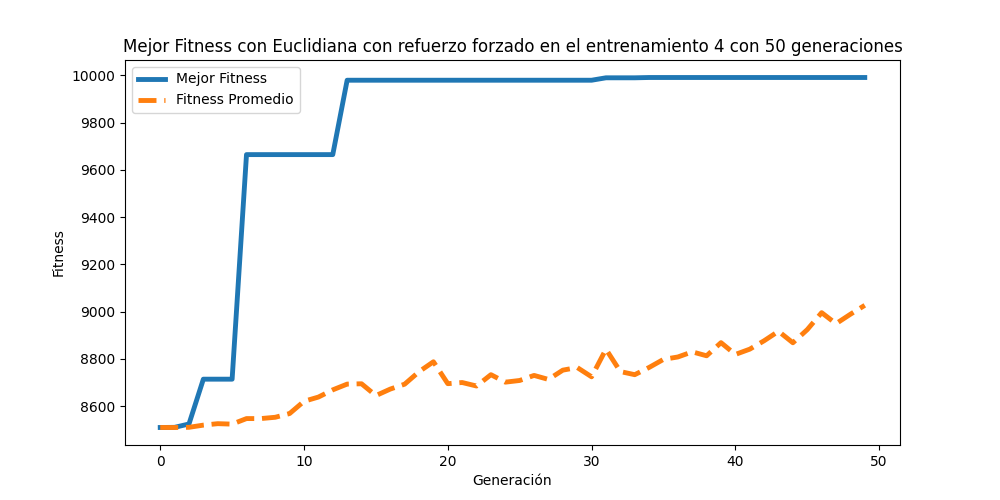
\includegraphics[width=0.9\linewidth]{Euclidiana/Fitnes_individual/Fitness_4_Eucli_50Gen.png}
    \caption{Fitness individual para el entrenamiento 4 de 50 generaciones aplicando la distancia Euclidiana}
    \label{fig:Fitnes_ecu_4_50_inv}
\end{figure}
\begin{figure}[H]
    \centering
    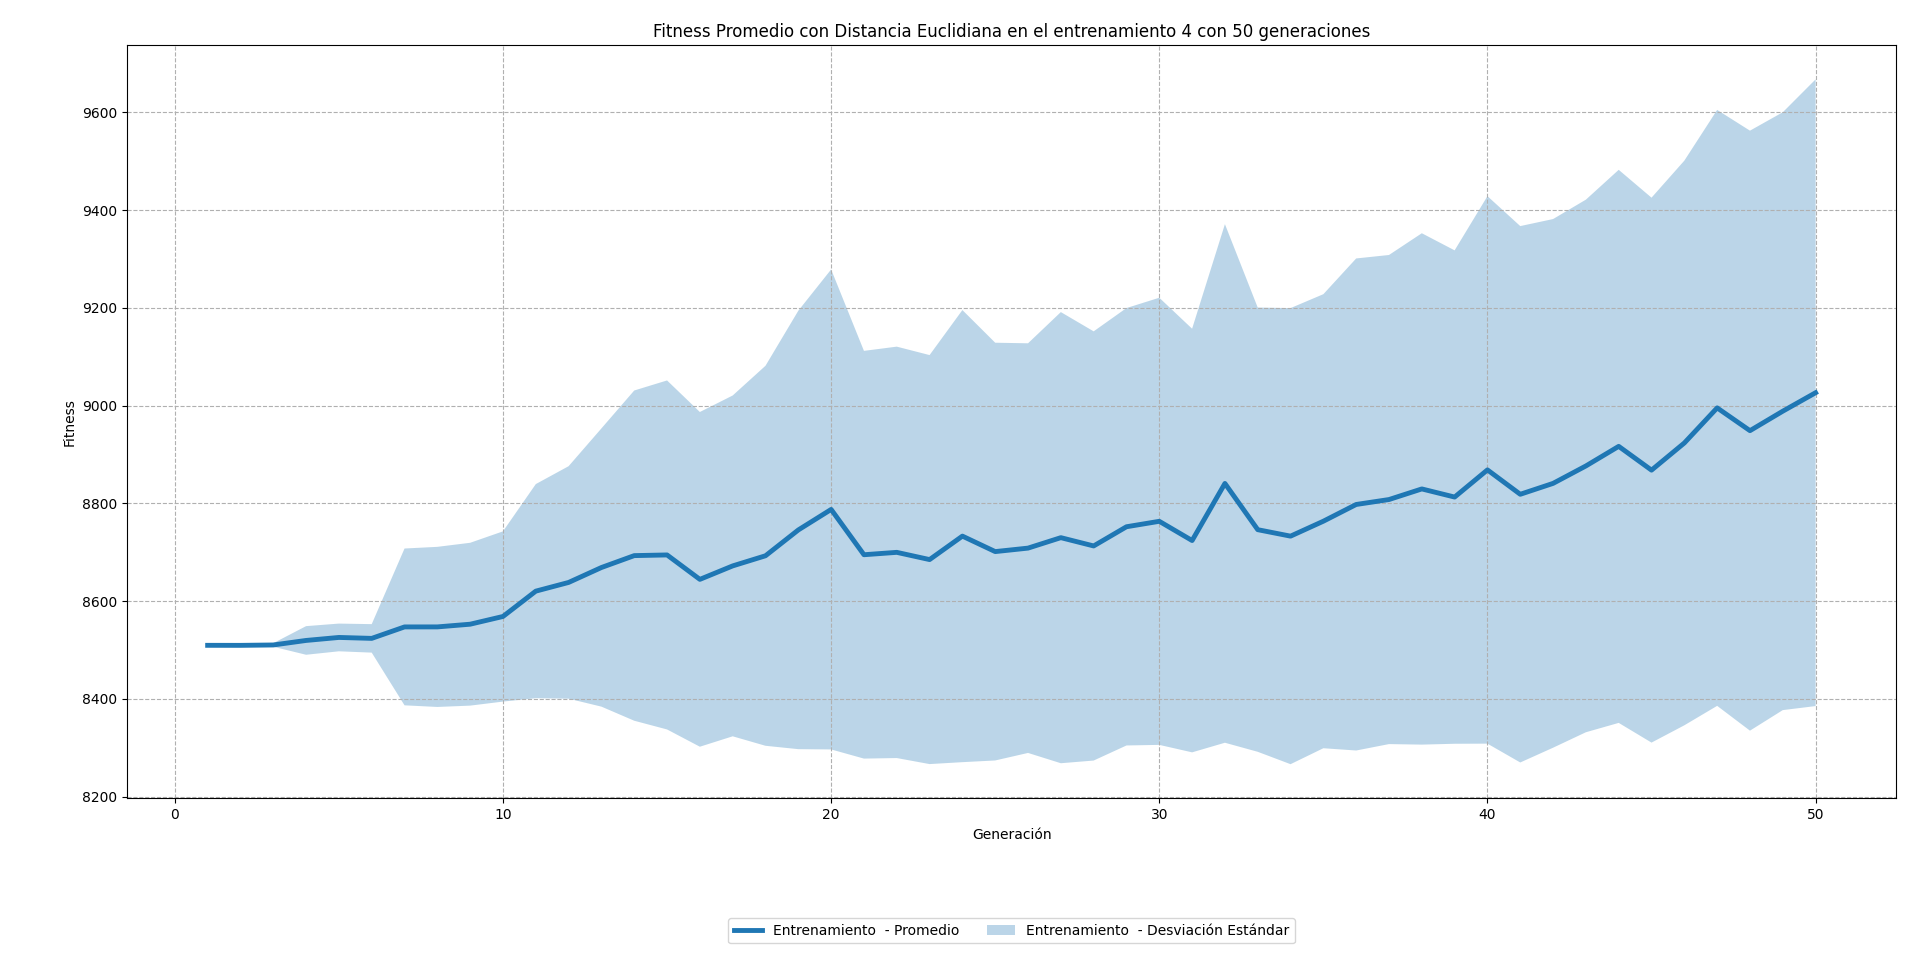
\includegraphics[width=0.9\linewidth]{Euclidiana/Fitnes_individual/Fitness_4_Eucli_50Gen_Sombra.png}
    \caption{Fitness promedio y desviación individual para el entrenamiento 4 de 50 generaciones aplicando la distancia Euclidiana}
    \label{fig:Fitnes_ecu_4_50_inv_sombra}
\end{figure}


\begin{figure}[H]
    \centering
    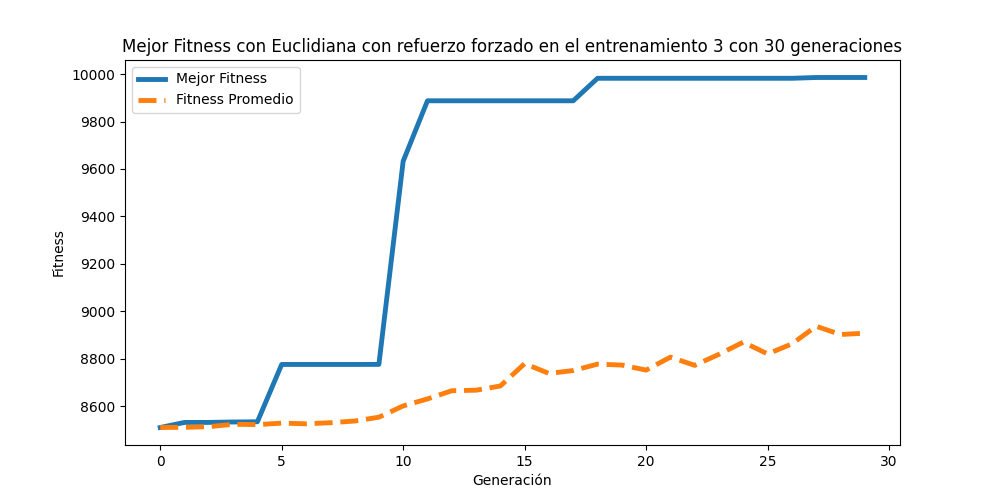
\includegraphics[width=0.9\linewidth]{Euclidiana/Fitness_individual_30/Fitness_3_Eucli_30Gen.png}
    \caption{Fitness individual para el entrenamiento 3 de 30 generaciones aplicando la distancia Euclidiana}
    \label{fig:Fitnes_ecu_3_30_inv}
\end{figure}

\begin{figure}[H]
    \centering
    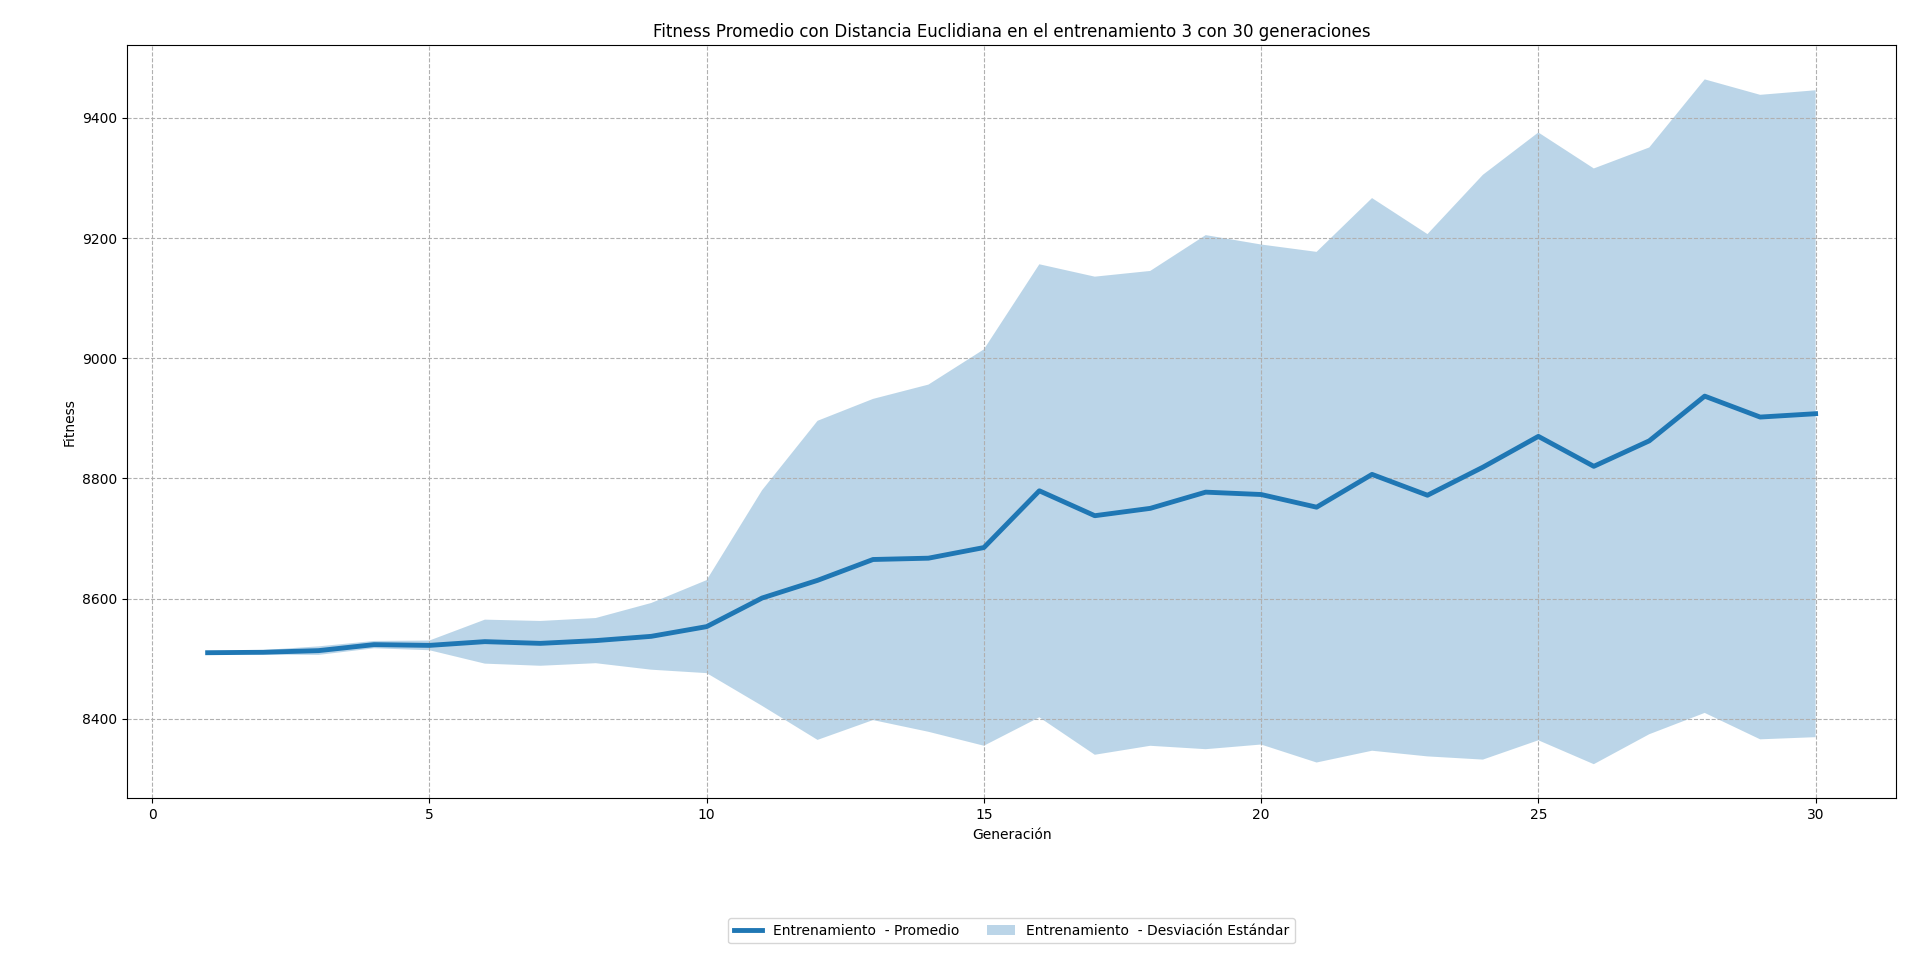
\includegraphics[width=0.9\linewidth]{Euclidiana/Fitness_individual_30/Fitness_3_Eucli_30Gen_Sombra.png}
    \caption{Fitness promedio y desviación individual para el entrenamiento 3 de 30 generaciones aplicando la distancia Euclidiana}
    \label{fig:Fitnes_ecu_3_30_inv_sombra}
\end{figure}








%%%------------------

\begin{figure}[H]
    \centering
    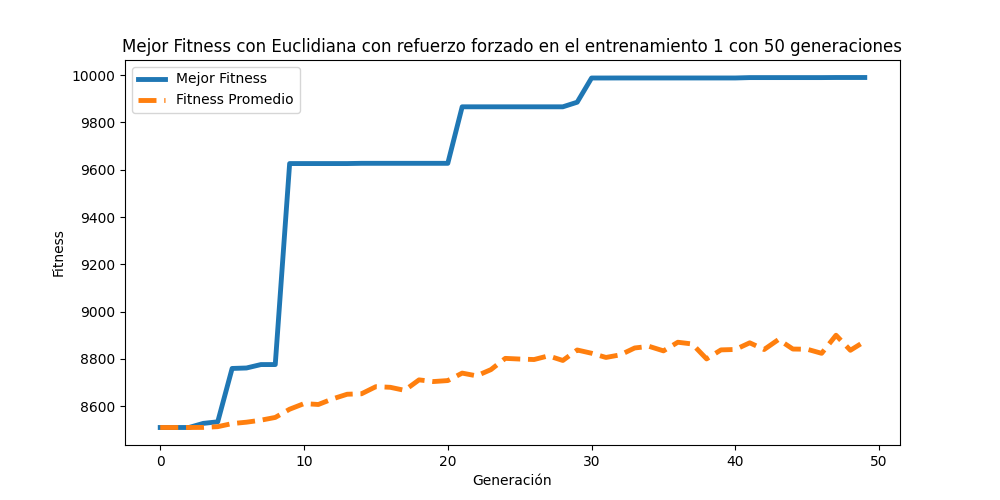
\includegraphics[width=0.9 \linewidth]{Euclidiana/Fitnes_individual/Fitness_1_Eucli_50Gen.png}
    \caption{Fitness individual para el entrenamiento 1 de 50 generaciones aplicando la distancia Euclidiana}
    \label{fig:eucli_1_50}
\end{figure}
\begin{figure}[H]
    \centering
    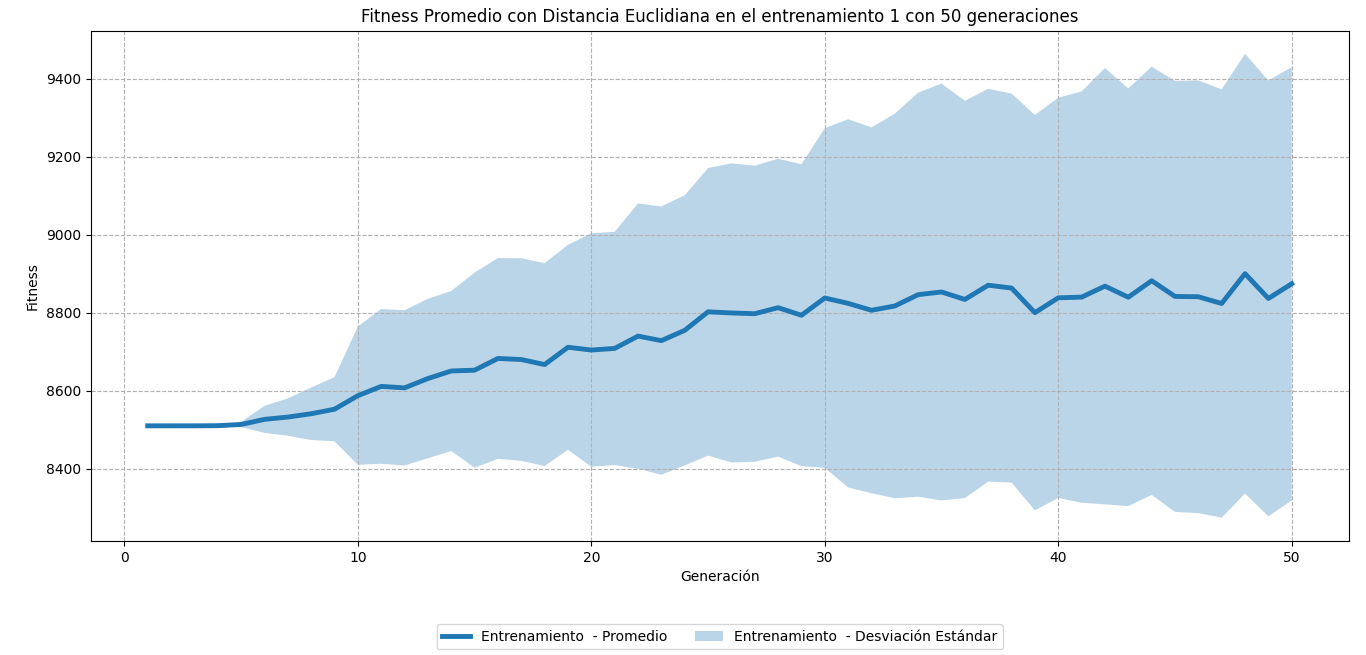
\includegraphics[width=0.9 \linewidth]{Euclidiana/Fitnes_individual/Fitness_1_Eucli_50Gen_Sombra.png}
    \caption{Fitness promedio y desviaciones para el entrenamiento 1 de 50 generaciones aplicando la distancia Euclidiana}
    \label{fig:eucli_1_50_sombra}
\end{figure}


\begin{figure}[H]
    \centering
    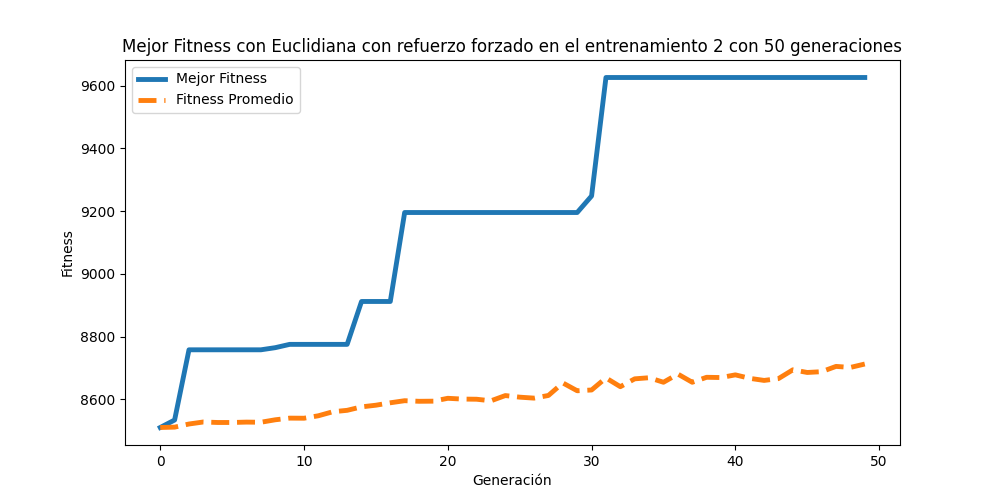
\includegraphics[width=0.9 \linewidth]{Euclidiana/Fitnes_individual/Fitness_2_Eucli_50Gen.png}
    \caption{Fitness individual para el entrenamiento 2 de 50 generaciones aplicando la distancia Euclidiana}
    \label{fig:eucli_2_50}
\end{figure}
\begin{figure}[H]
    \centering
    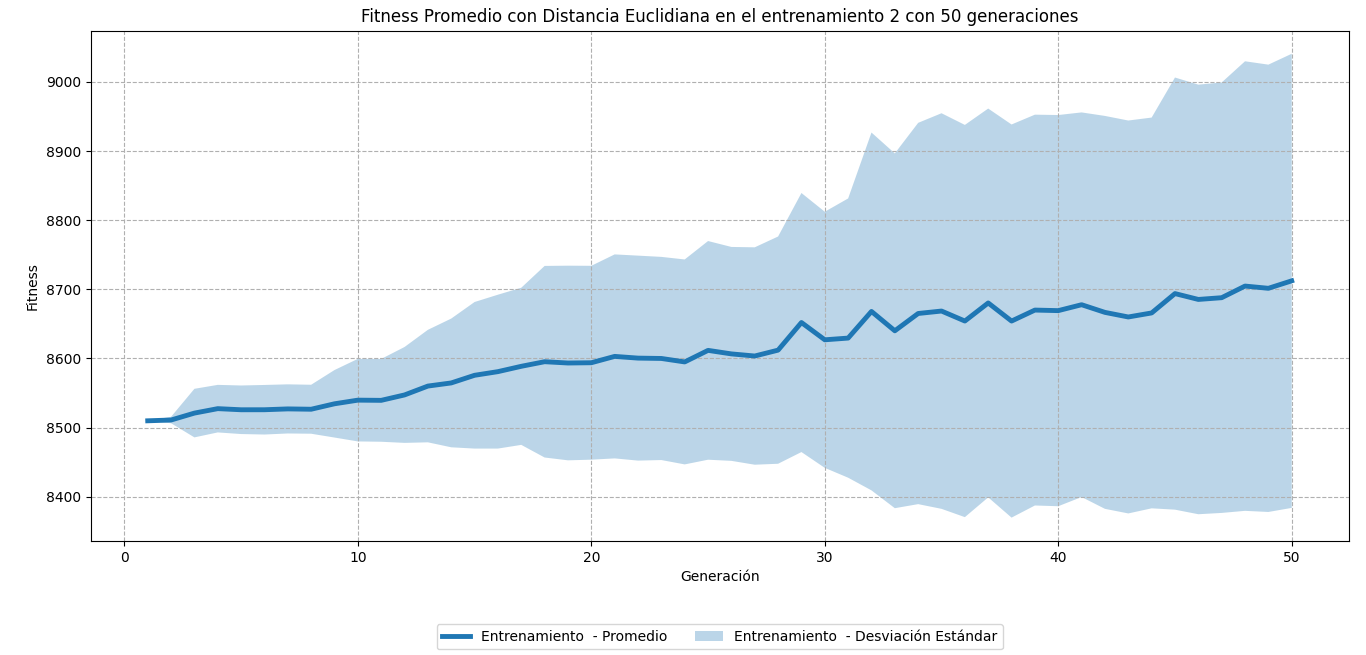
\includegraphics[width=0.9 \linewidth]{Euclidiana/Fitnes_individual/Fitness_2_Eucli_50Gen_Sombra.png}
    \caption{Fitness promedio y desviaciones para el entrenamiento 2 de 50 generaciones aplicando la distancia Euclidiana}
    \label{fig:eucli_2_50_sombra}
\end{figure}

\begin{figure}[H]
    \centering
    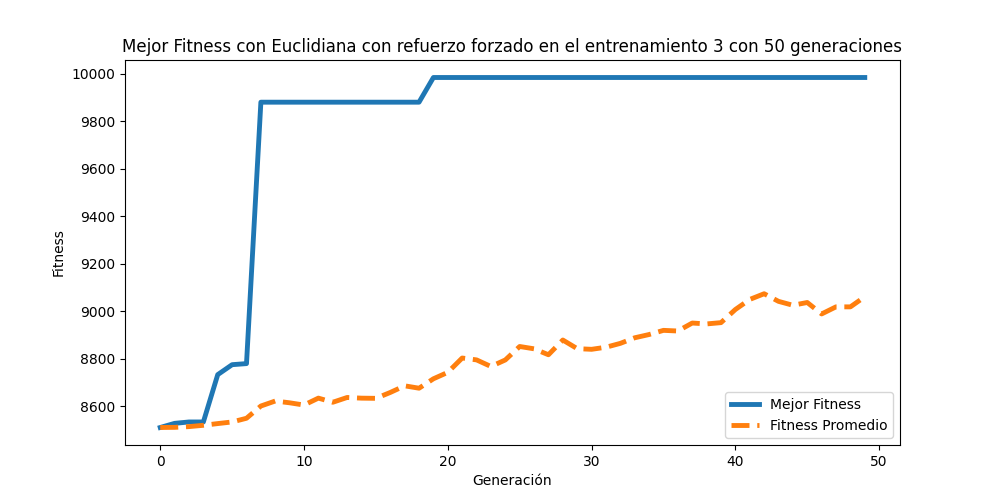
\includegraphics[width=0.9 \linewidth]{Euclidiana/Fitnes_individual/Fitness_3_Eucli_50Gen.png}
    \caption{Fitness individual para el entrenamiento 3 de 50 generaciones aplicando la distancia Euclidiana}
    \label{fig:eucli_3_50}
\end{figure}
\begin{figure}[H]
    \centering
    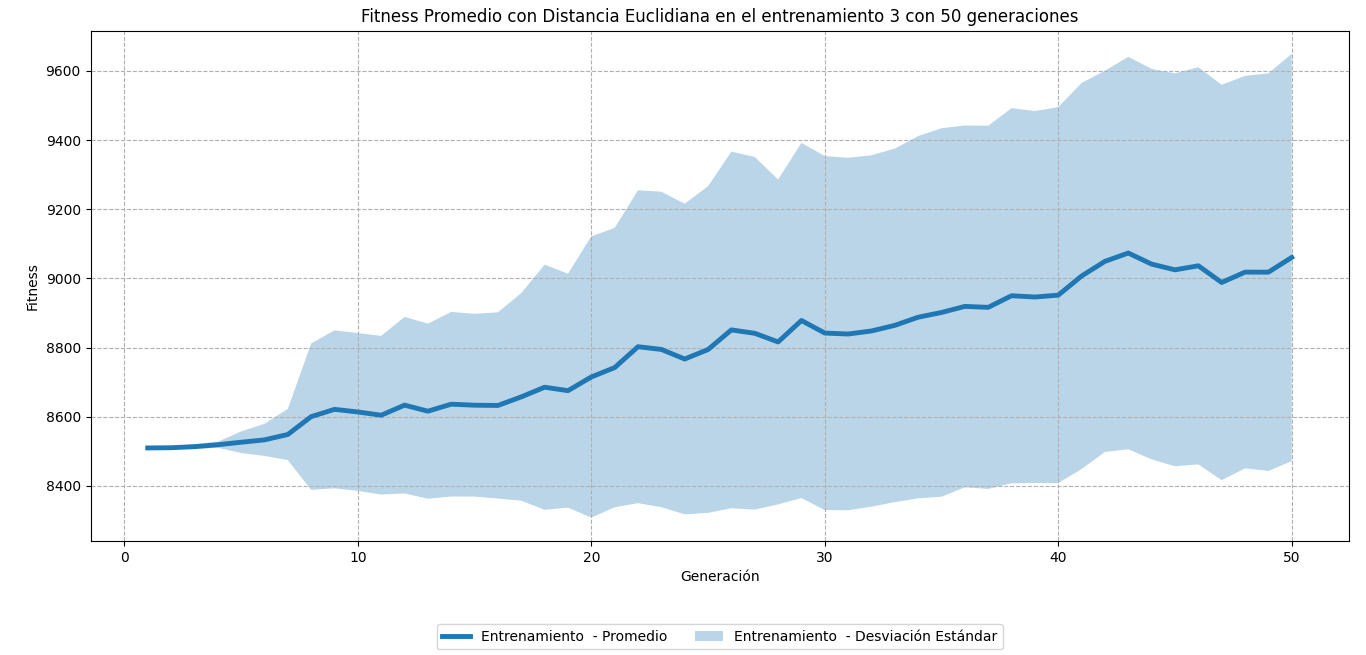
\includegraphics[width=0.9 \linewidth]{Euclidiana/Fitnes_individual/Fitness_3_Eucli_50Gen_Sombra.png}
    \caption{Fitness promedio y desviaciones para el entrenamiento 3 de 50 generaciones aplicando la distancia Euclidiana}
    \label{fig:eucli_3_50_sombra}
\end{figure}

\begin{figure}[H]
    \centering
    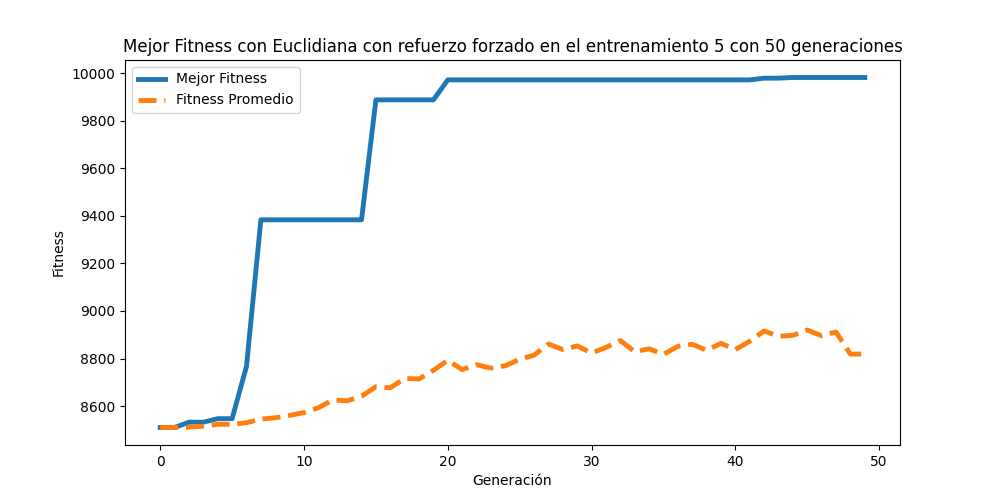
\includegraphics[width=0.9 \linewidth]{Euclidiana/Fitnes_individual/Fitness_5_Eucli_50Gen.png}
    \caption{Fitness individual para el entrenamiento 5 de 50 generaciones aplicando la distancia Euclidiana}
    \label{fig:eucli_5_50}
\end{figure}
\begin{figure}[H]
    \centering
    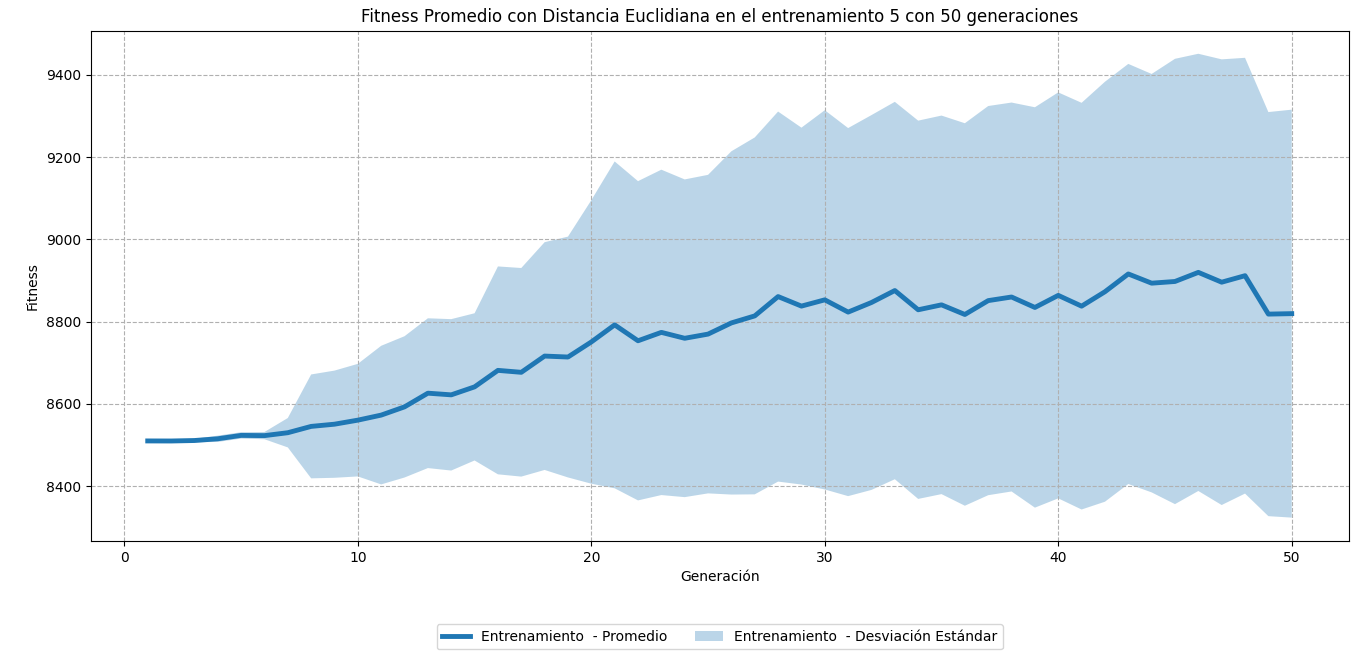
\includegraphics[width=0.9 \linewidth]{Euclidiana/Fitnes_individual/Fitness_5_Eucli_50Gen_Sombra.png}
    \caption{Fitness promedio y desviaciones para el entrenamiento 5 de 50 generaciones aplicando la distancia Euclidiana}
    \label{fig:eucli_5_50_sombra}
\end{figure}

\subsection{Generación 30}
\setcounter{figure}{0}
\renewcommand{\thefigure}{S\arabic{figure}B-E}
% Eucli30Gen
% 1 9981
% 2 9883
% 3 9986
% 4 8544
% 5 9984
\begin{figure}[H]
    \centering
    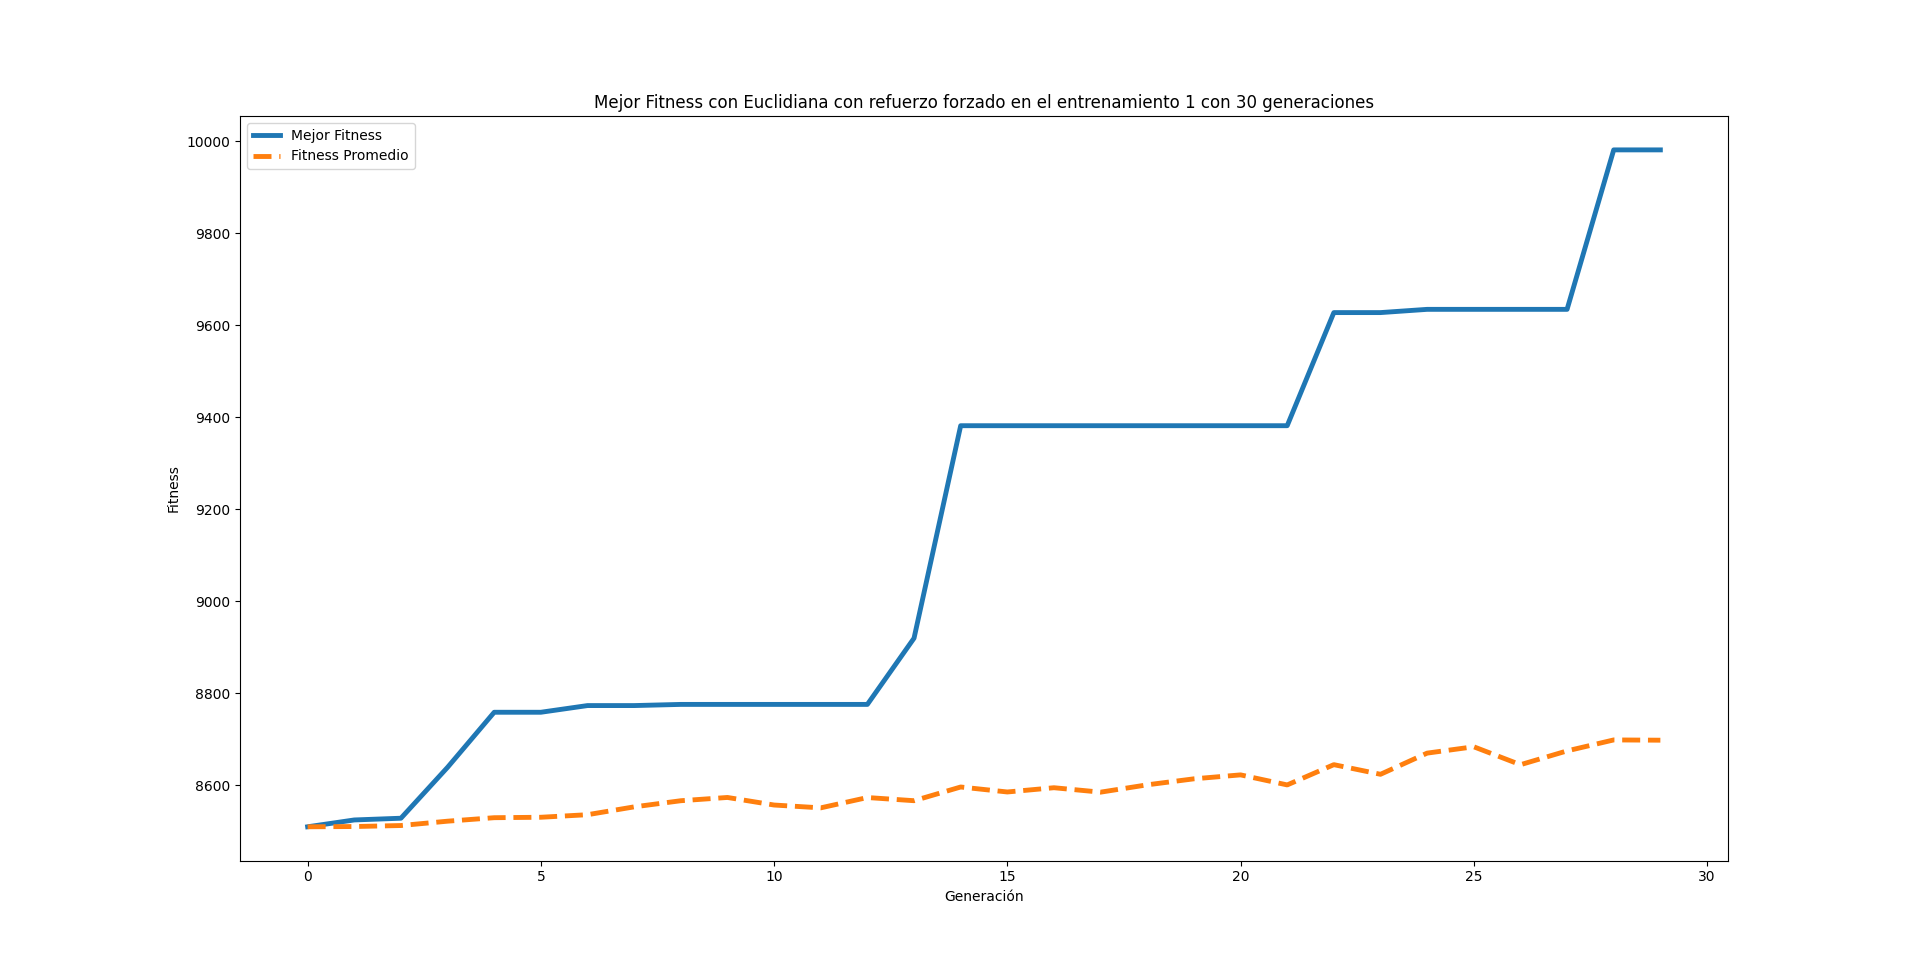
\includegraphics[width=0.9 \linewidth]{Euclidiana/Fitness_individual_30/Fitness_1_Eucli_30Gen.png}
    \caption{Fitness individual para el entrenamiento 1 de 30 generaciones aplicando la distancia Euclidiana}
    \label{fig:eucli_1_30}
\end{figure}
\begin{figure}[H]
    \centering
    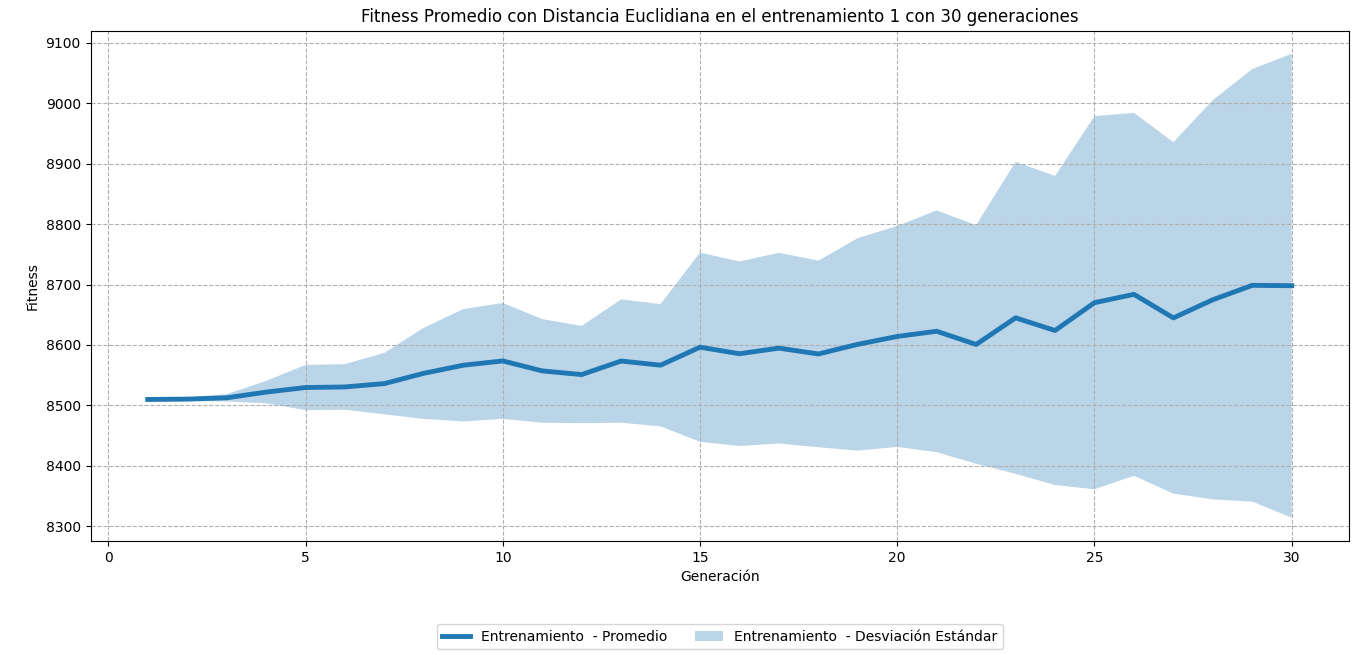
\includegraphics[width=0.9 \linewidth]{Euclidiana/Fitness_individual_30/Fitness_1_Eucli_30Gen_Sombra.png}
    \caption{Fitness promedio y desviaciones para el entrenamiento 1 de 30 generaciones aplicando la distancia Euclidiana}
    \label{fig:eucli_1_30_sombra}
\end{figure}

\begin{figure}[H]
    \centering
    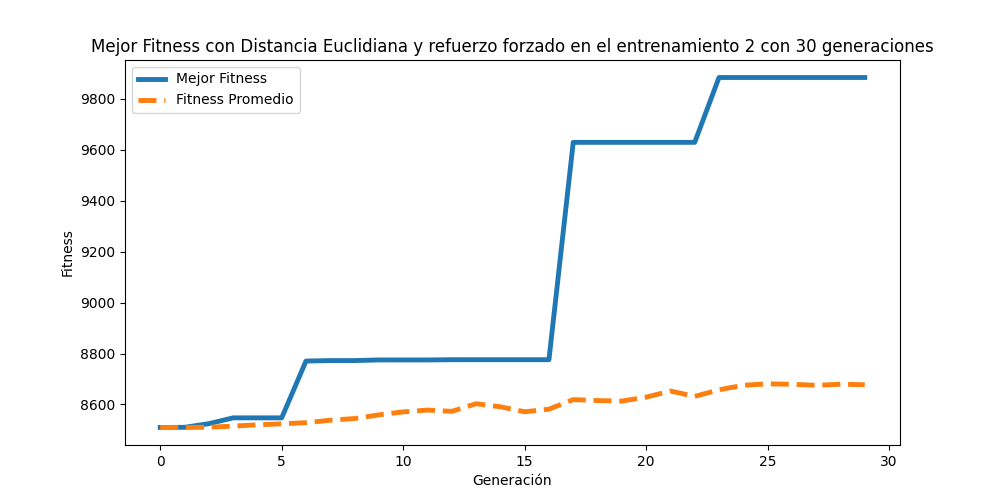
\includegraphics[width=0.9 \linewidth]{Euclidiana/Fitness_individual_30/Fitness_2_Eucli_30Gen.png}
    \caption{Fitness individual para el entrenamiento 2 de 30 generaciones aplicando la distancia Euclidiana}
    \label{fig:eucli_2_30}
\end{figure}
\begin{figure}[H]
    \centering
    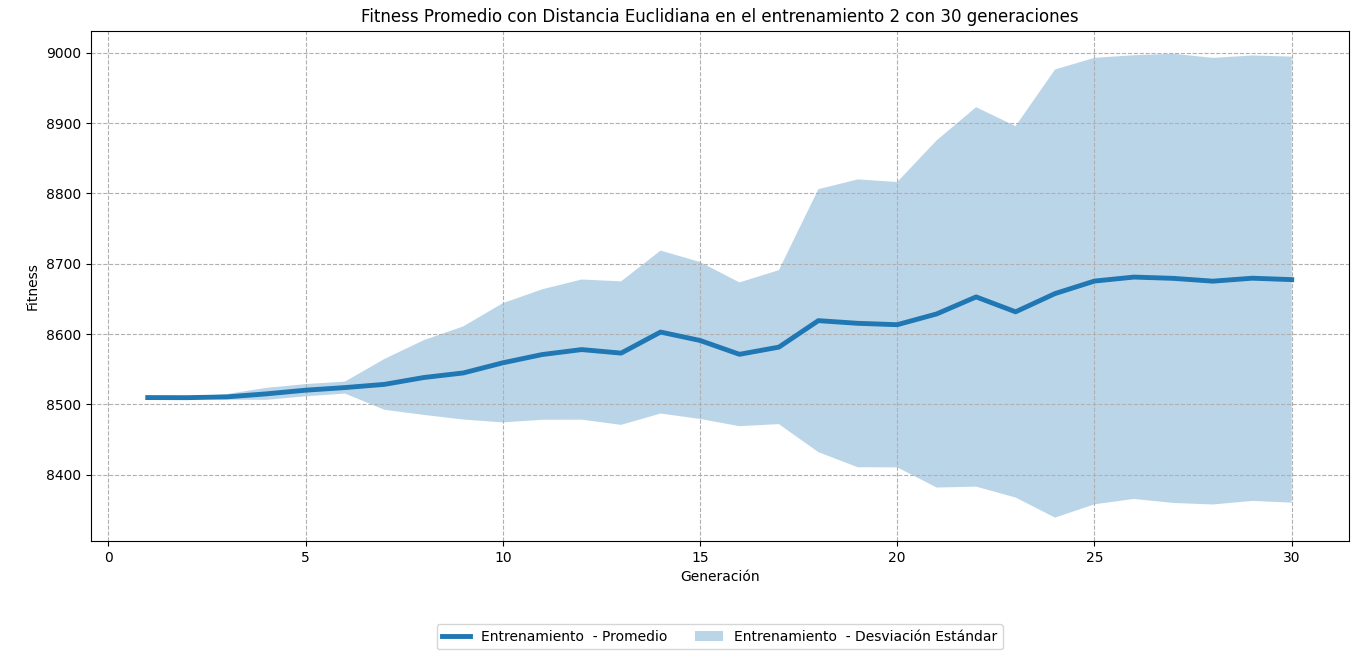
\includegraphics[width=0.9 \linewidth]{Euclidiana/Fitness_individual_30/Fitness_2_Eucli_30Gen_Sombra.png}
    \caption{Fitness promedio y desviaciones para el entrenamiento 2 de 30 generaciones aplicando la distancia Euclidiana}
    \label{fig:eucli_2_30_sombra}
\end{figure}

\begin{figure}[H]
    \centering
    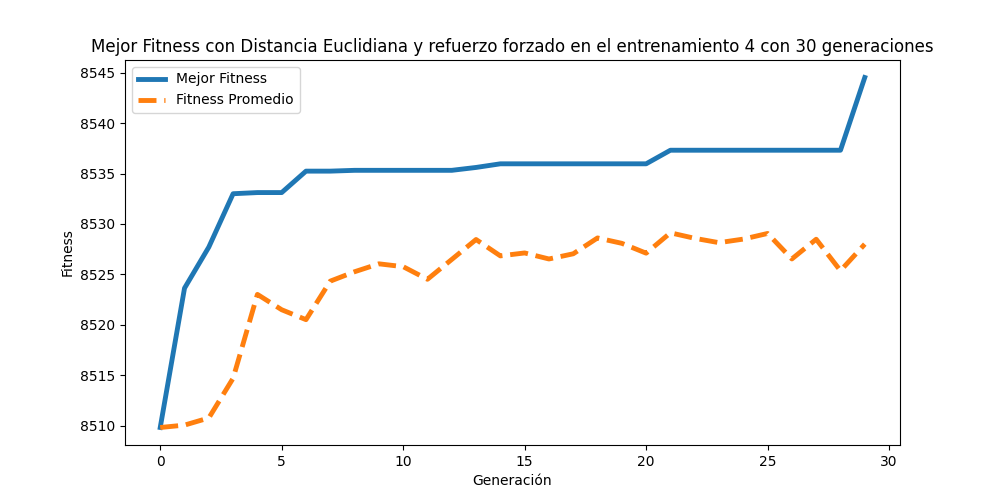
\includegraphics[width=0.9 \linewidth]{Euclidiana/Fitness_individual_30/Fitness_4_Eucli_30Gen.png}
    \caption{Fitness individual para el entrenamiento 2 de 30 generaciones aplicando la distancia Euclidiana}
    \label{fig:eucli_4_30}
\end{figure}
\begin{figure}[H]
    \centering
    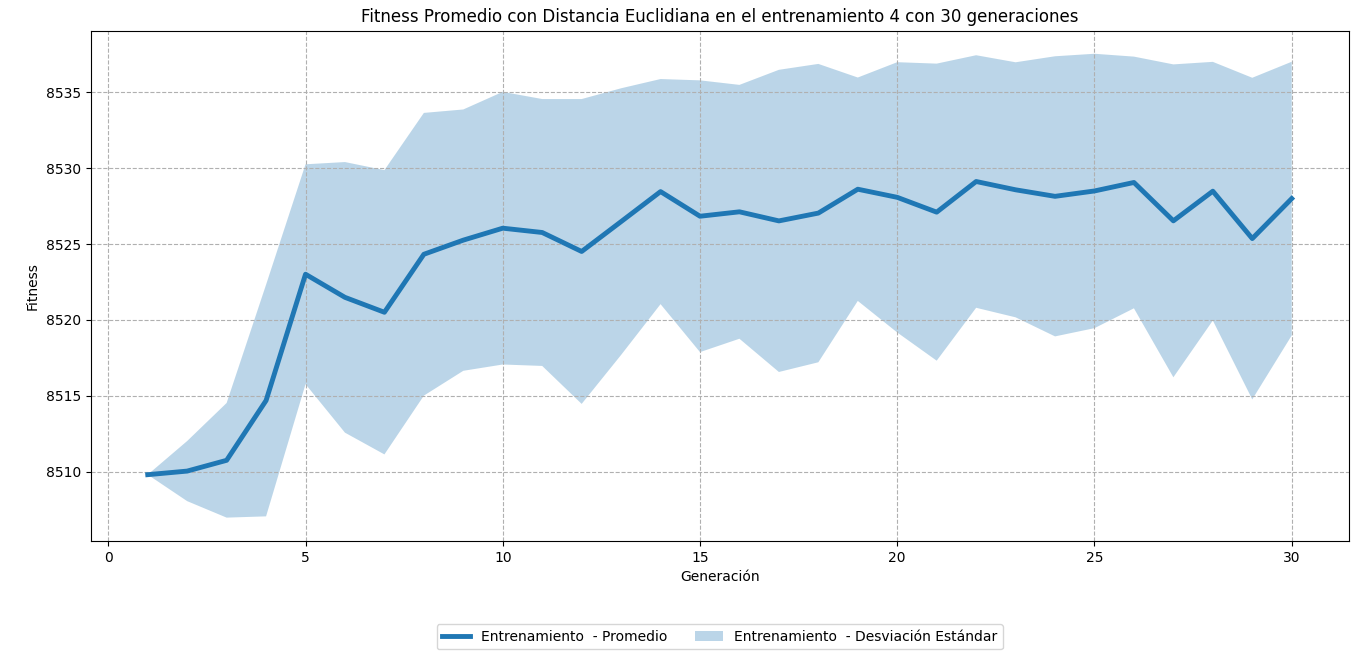
\includegraphics[width=0.9 \linewidth]{Euclidiana/Fitness_individual_30/Fitness_4_Eucli_30Gen_Sombra.png}
    \caption{Fitness promedio y desviaciones para el entrenamiento 2 de 30 generaciones aplicando la distancia Euclidiana}
    \label{fig:eucli_4_30_sombra}
\end{figure}

\begin{figure}[H]
    \centering
    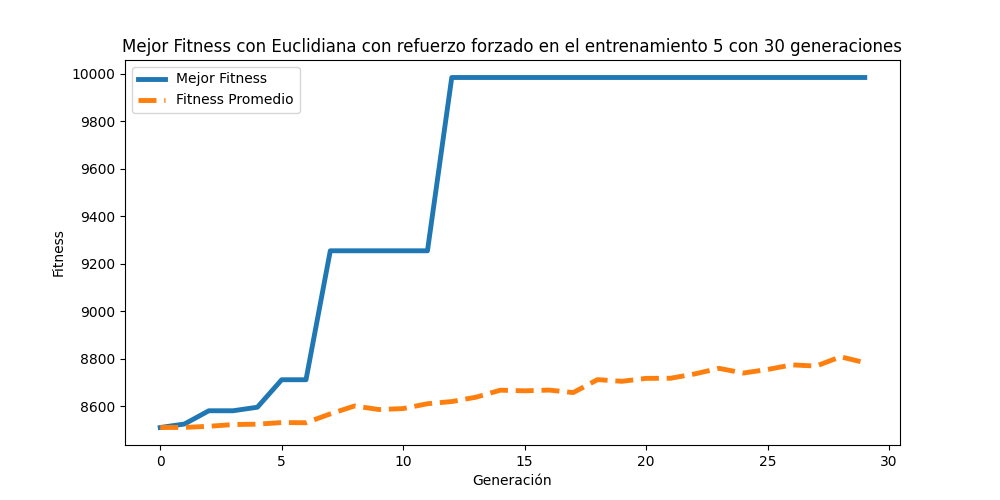
\includegraphics[width=0.9 \linewidth]{Euclidiana/Fitness_individual_30/Fitness_5_Eucli_30Gen.png}
    \caption{Fitness individual para el entrenamiento 5 de 30 generaciones aplicando la distancia Euclidiana}
    \label{fig:eucli_5_30}
\end{figure}
\begin{figure}[H]
    \centering
    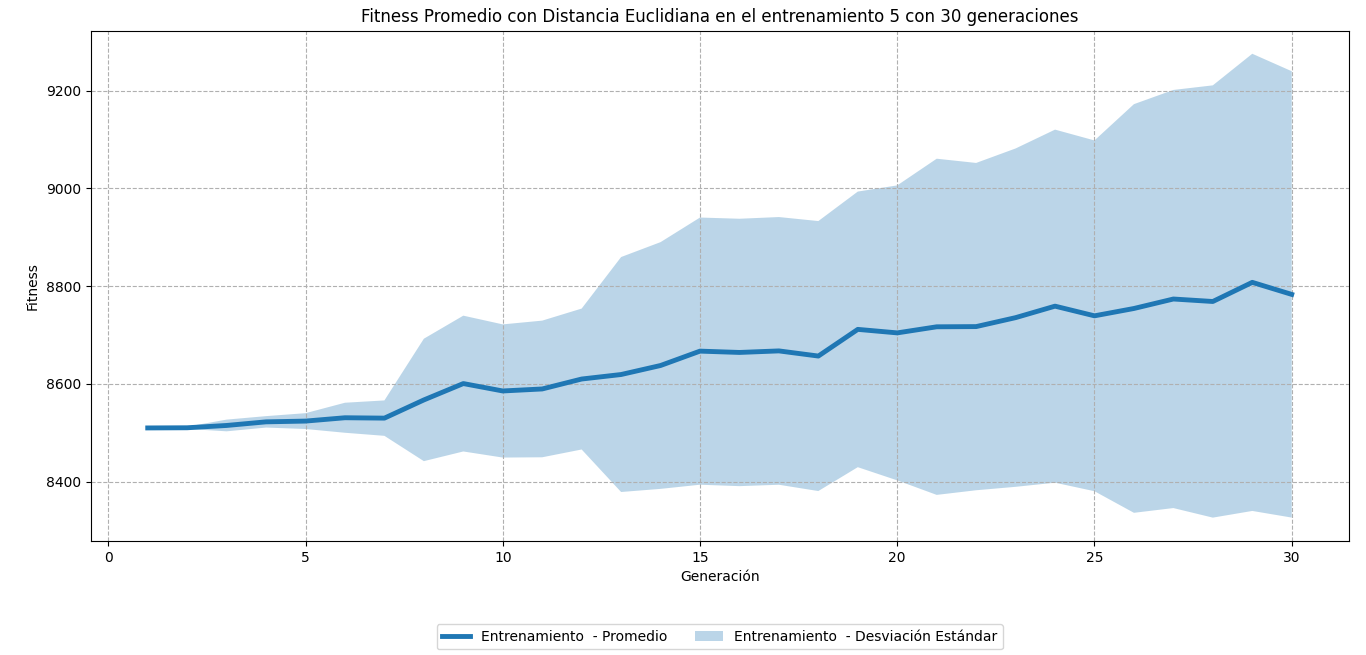
\includegraphics[width=0.9 \linewidth]{Euclidiana/Fitness_individual_30/Fitness_5_Eucli_30Gen_Sombra.png}
    \caption{Fitness promedio y desviaciones para el entrenamiento 5 de 30 generaciones aplicando la distancia Euclidiana}
    \label{fig:eucli_5_30_sombra}
\end{figure}


\subsection{Generación 20}
\setcounter{figure}{0}
\renewcommand{\thefigure}{S\arabic{figure}C-E}
% Eucli20Gen
% 1 9632
% 2 9881
% 3 8773
% 4 9237
% 5 8782
\begin{figure}[H]
    \centering
    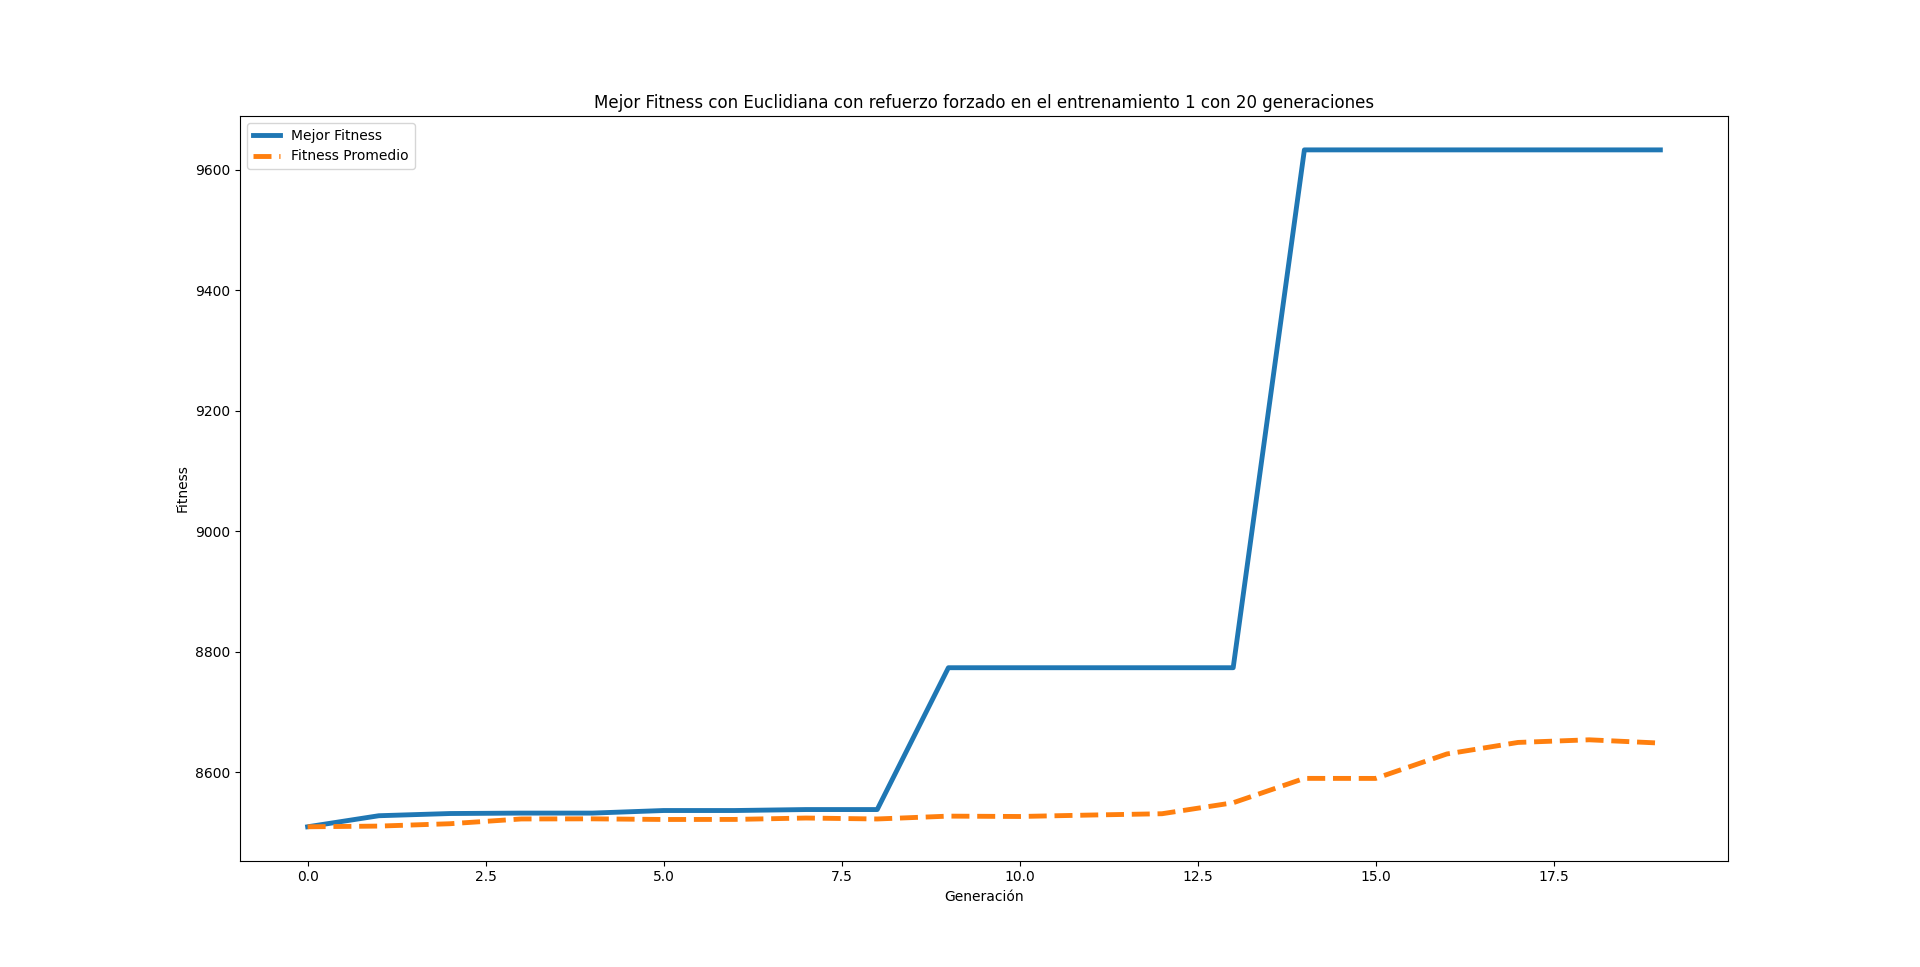
\includegraphics[width=0.9 \linewidth]{Euclidiana/Fitness_individual_20/Fitness_1_Eucli_20Gen.png}
    \caption{Fitness individual para el entrenamiento 1 de 20 generaciones aplicando la distancia Euclidiana}
    \label{fig:eucli_1_20}
\end{figure}
\begin{figure}[H]
    \centering
    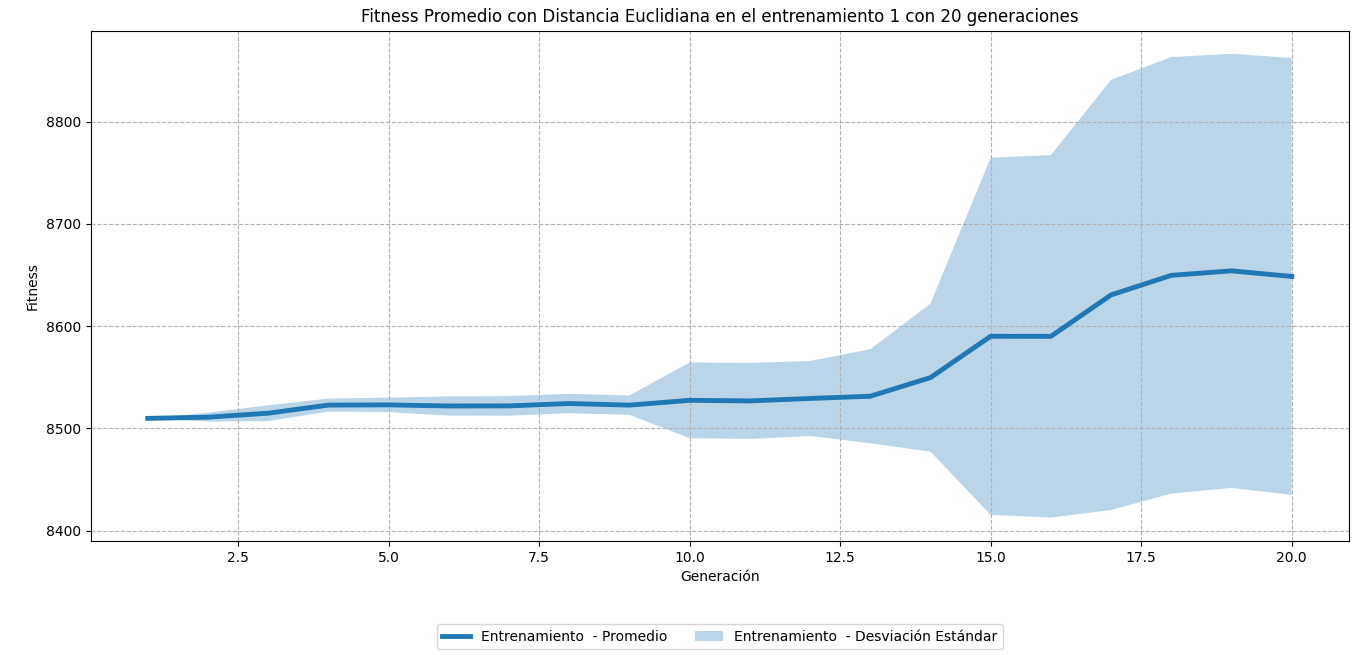
\includegraphics[width=0.9 \linewidth]{Euclidiana/Fitness_individual_20/Fitness_1_Eucli_20Gen_Sombra.png}
    \caption{Fitness promedio y desviaciones para el entrenamiento 1 de 20 generaciones aplicando la distancia Euclidiana}
    \label{fig:eucli_1_20_sombra}
\end{figure}

\begin{figure}[H]
    \centering
    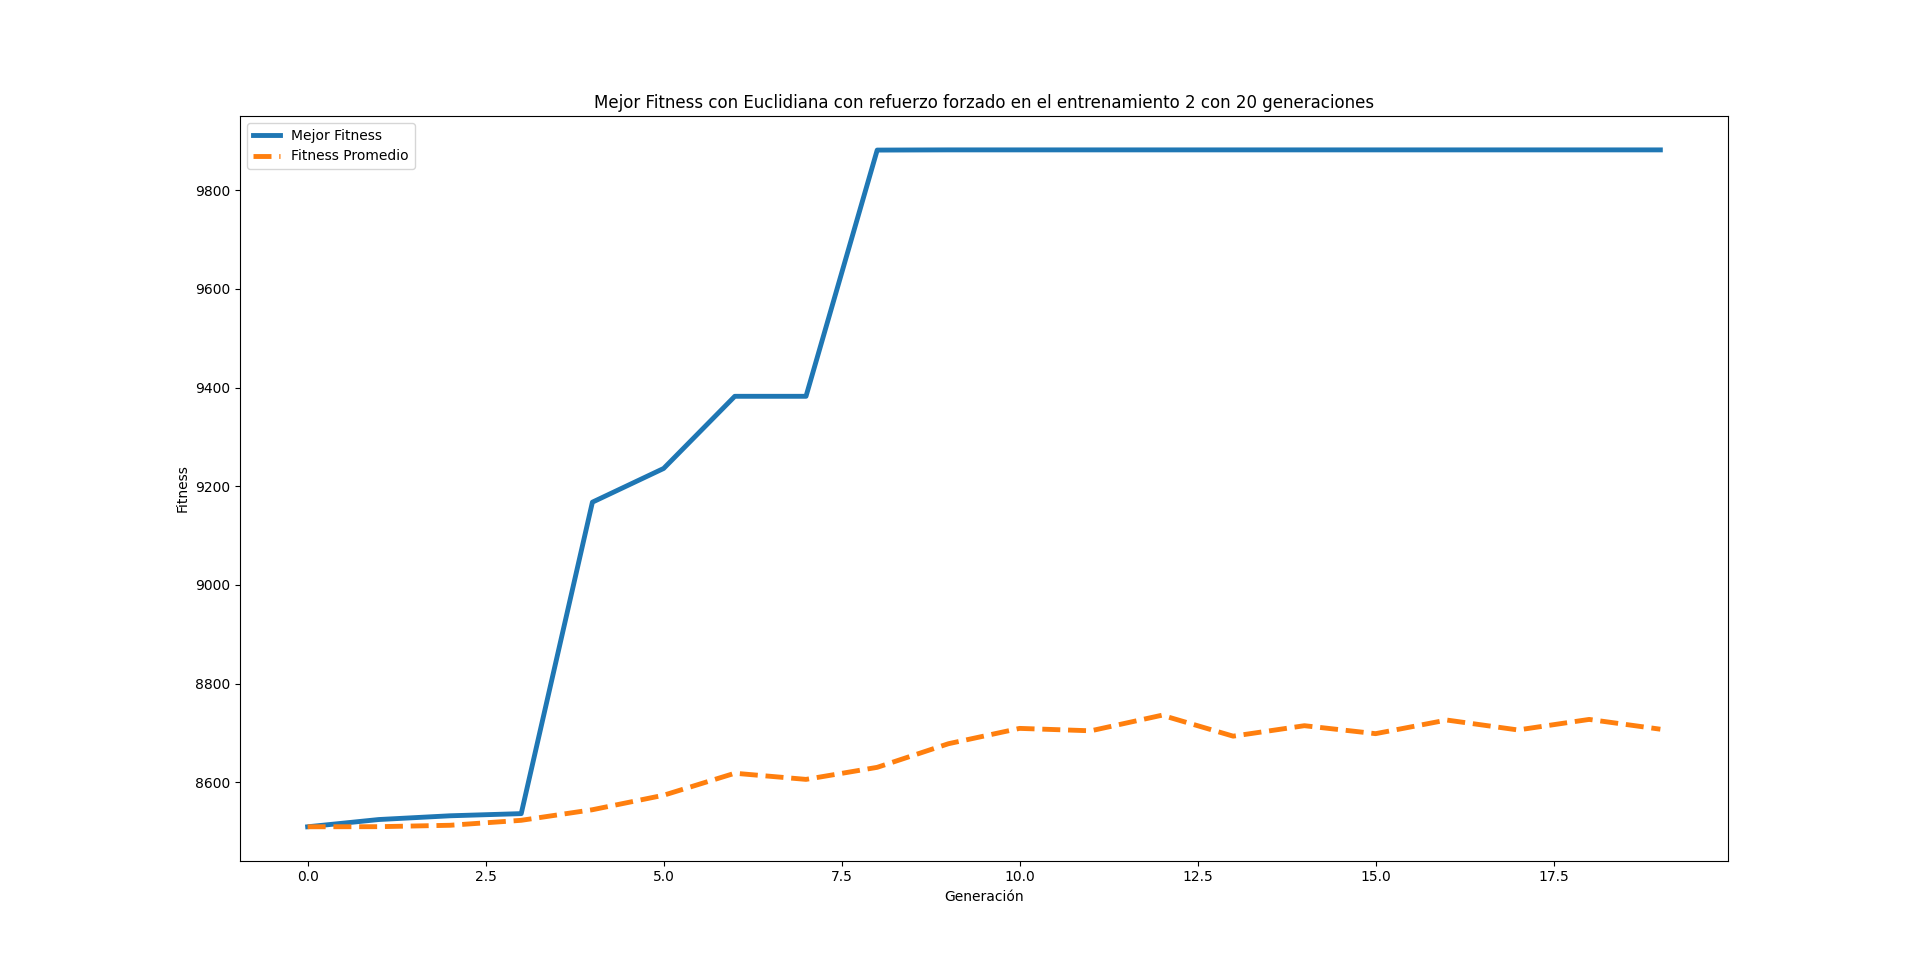
\includegraphics[width=0.9 \linewidth]{Euclidiana/Fitness_individual_20/Fitness_2_Eucli_20Gen.png}
    \caption{Fitness individual para el entrenamiento 2 de 20 generaciones aplicando la distancia Euclidiana}
    \label{fig:eucli_2_20}
\end{figure}
\begin{figure}[H]
    \centering
    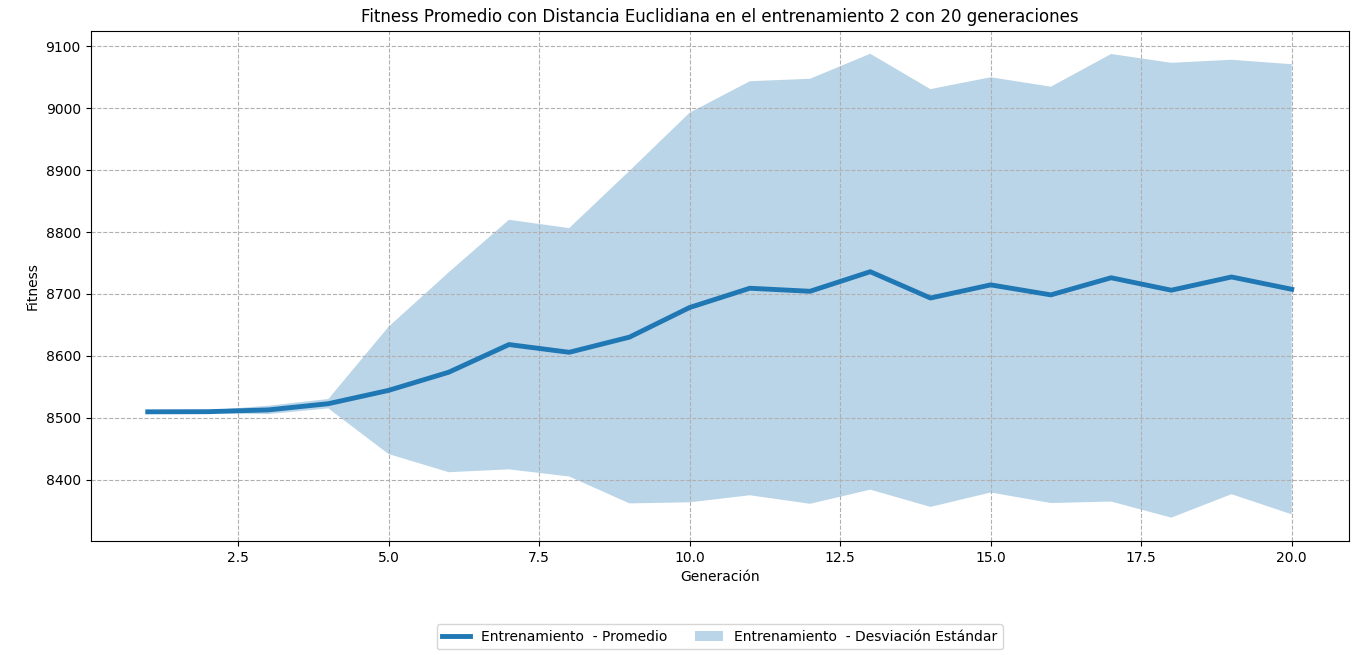
\includegraphics[width=0.9 \linewidth]{Euclidiana/Fitness_individual_20/Fitness_2_Eucli_20Gen_Sombra.png}
    \caption{Fitness promedio y desviaciones para el entrenamiento 2 de 20 generaciones aplicando la distancia Euclidiana}
    \label{fig:eucli_2_20_sombra}
\end{figure}

\begin{figure}[H]
    \centering
    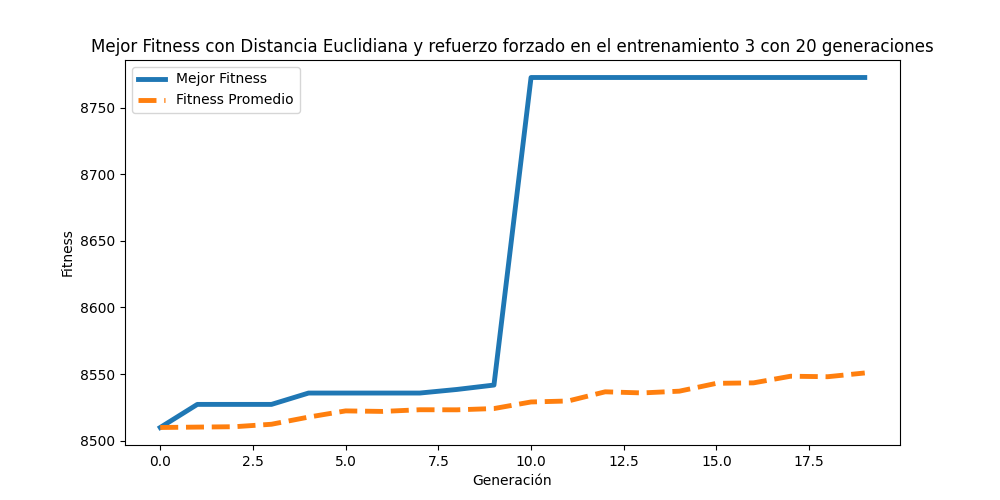
\includegraphics[width=0.9 \linewidth]{Euclidiana/Fitness_individual_20/Fitness_3_Eucli_20Gen.png}
    \caption{Fitness individual para el entrenamiento 3 de 20 generaciones aplicando la distancia Euclidiana}
    \label{fig:eucli_3_20}
\end{figure}
\begin{figure}[H]
    \centering
    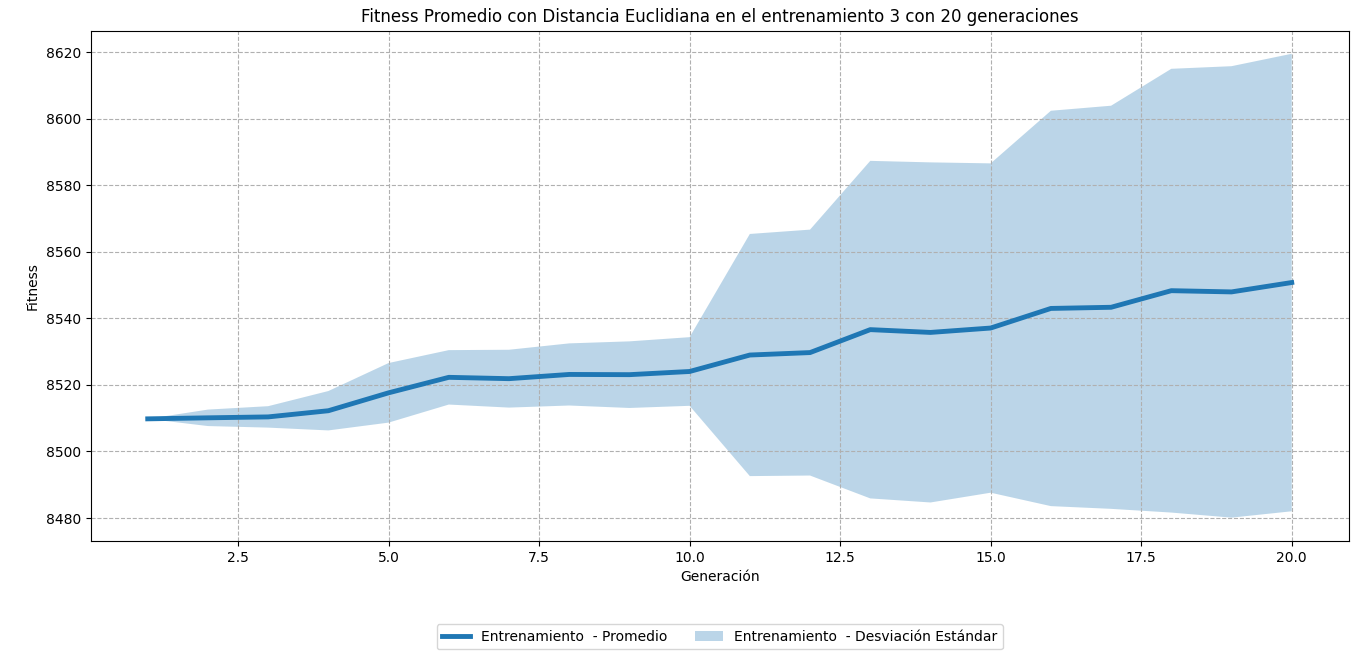
\includegraphics[width=0.9 \linewidth]{Euclidiana/Fitness_individual_20/Fitness_3_Eucli_20Gen_Sombra.png}
    \caption{Fitness promedio y desviaciones para el entrenamiento 3 de 20 generaciones aplicando la distancia Euclidiana}
    \label{fig:eucli_3_20_sombra}
\end{figure}

\begin{figure}[H]
    \centering
    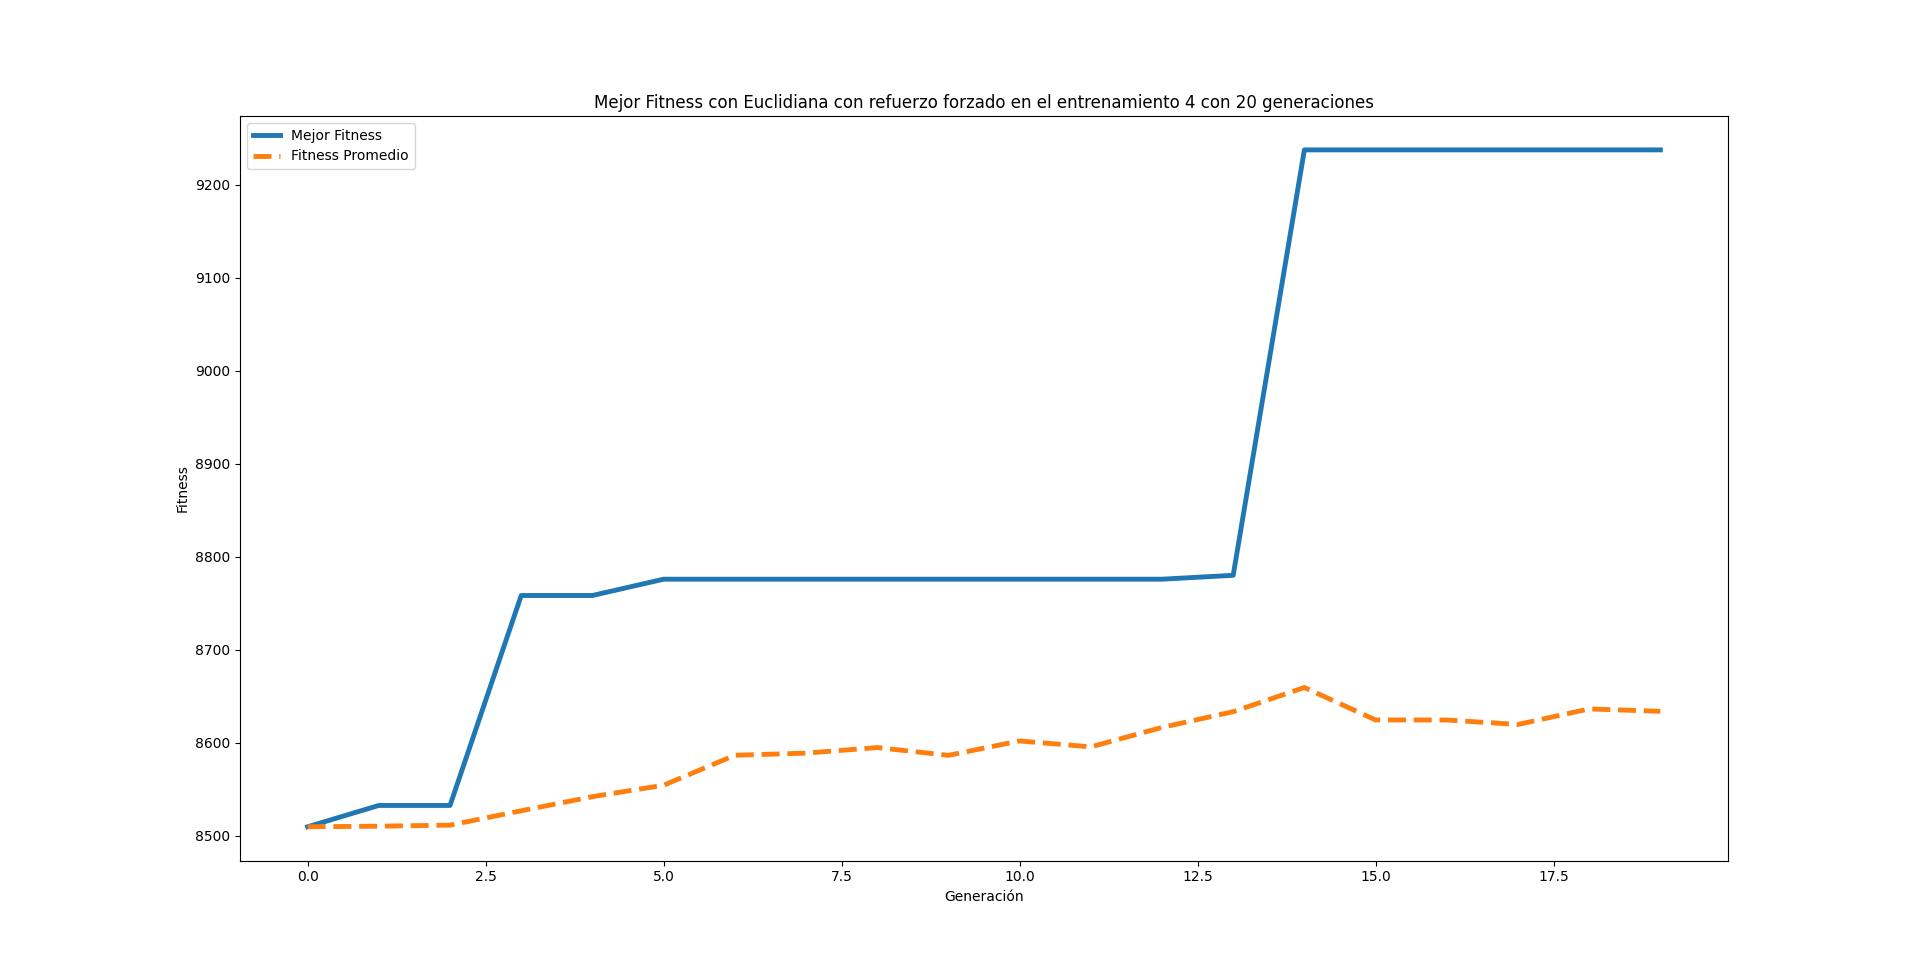
\includegraphics[width=0.9 \linewidth]{Euclidiana/Fitness_individual_20/Fitness_4_Eucli_20Gen.png}
    \caption{Fitness individual para el entrenamiento 4 de 20 generaciones aplicando la distancia Euclidiana}
    \label{fig:eucli_4_20}
\end{figure}
\begin{figure}[H]
    \centering
    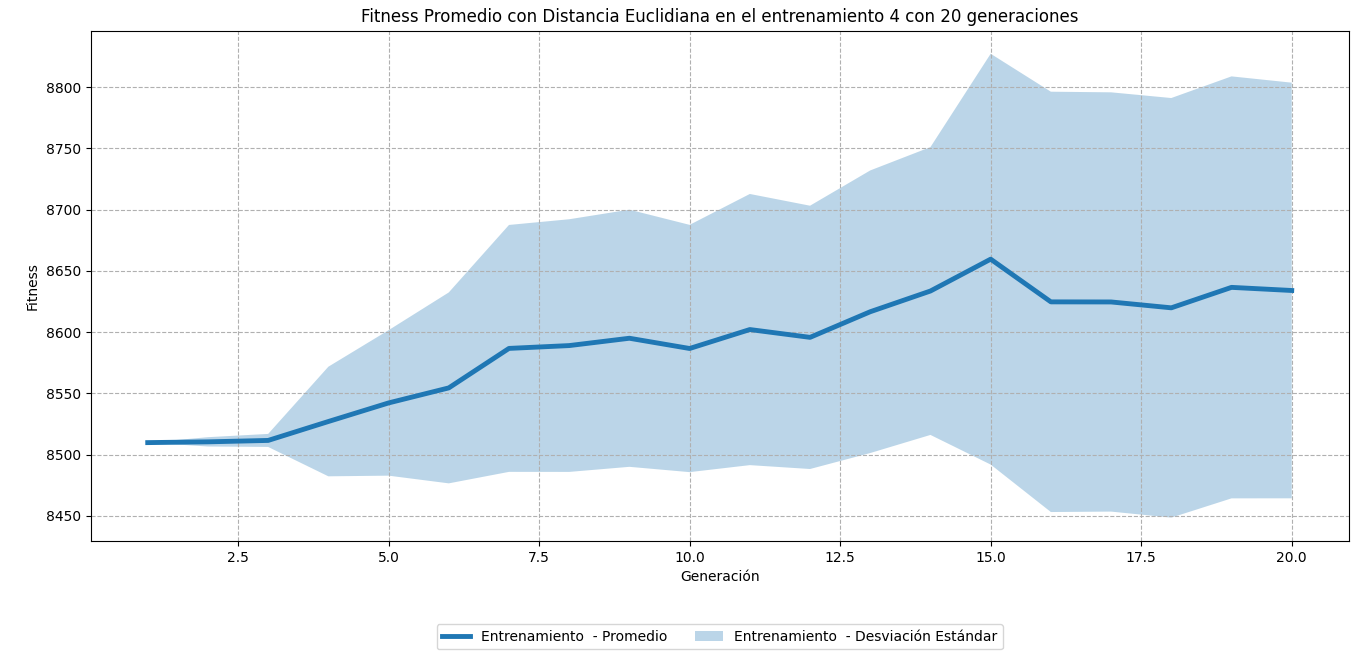
\includegraphics[width=0.9 \linewidth]{Euclidiana/Fitness_individual_20/Fitness_4_Eucli_20Gen_Sombra.png}
    \caption{Fitness promedio y desviaciones para el entrenamiento 4 de 20 generaciones aplicando la distancia Euclidiana}
    \label{fig:eucli_4_20_sombra}
\end{figure}

\begin{figure}[H]
    \centering
    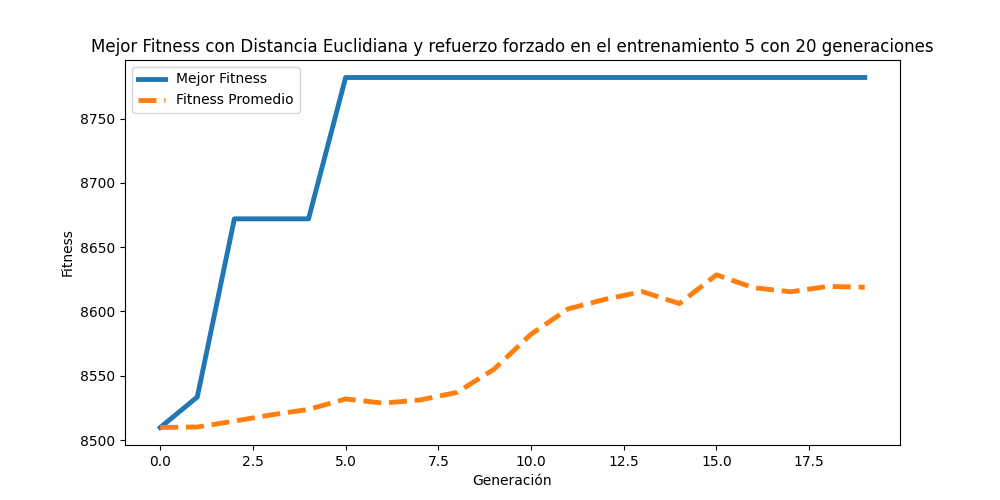
\includegraphics[width=0.9 \linewidth]{Euclidiana/Fitness_individual_20/Fitness_5_Eucli_20Gen.png}
    \caption{Fitness individual para el entrenamiento 5 de 20 generaciones aplicando la distancia Euclidiana}
    \label{fig:eucli_5_20}
\end{figure}
\begin{figure}[H]
    \centering
    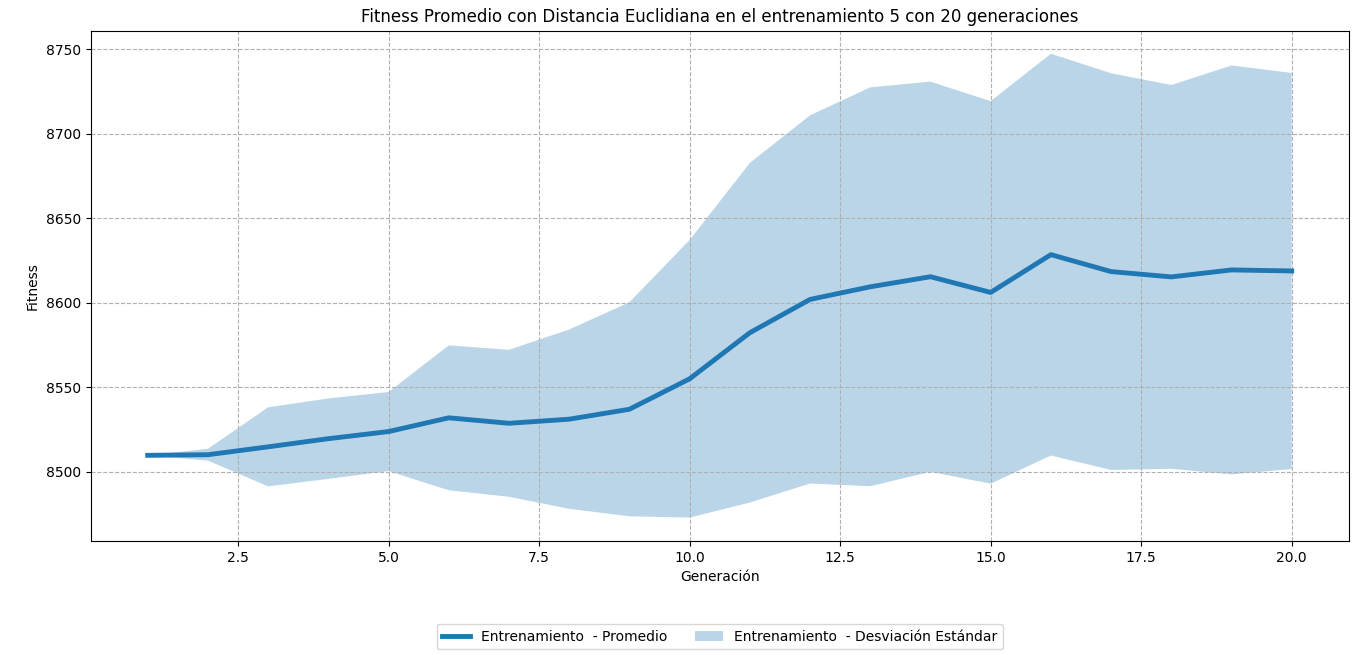
\includegraphics[width=0.9 \linewidth]{Euclidiana/Fitness_individual_20/Fitness_5_Eucli_20Gen_Sombra.png}
    \caption{Fitness promedio y desviaciones para el entrenamiento 5 de 20 generaciones aplicando la distancia Euclidiana}
    \label{fig:eucli_5_20_sombra}
\end{figure}

\section{Resultados de las simulaciones para la distancia Manhattan}
\subsection{Generación 50}
\setcounter{figure}{0}
\renewcommand{\thefigure}{S\arabic{figure}A-M}
\begin{figure}[H]
    \centering
    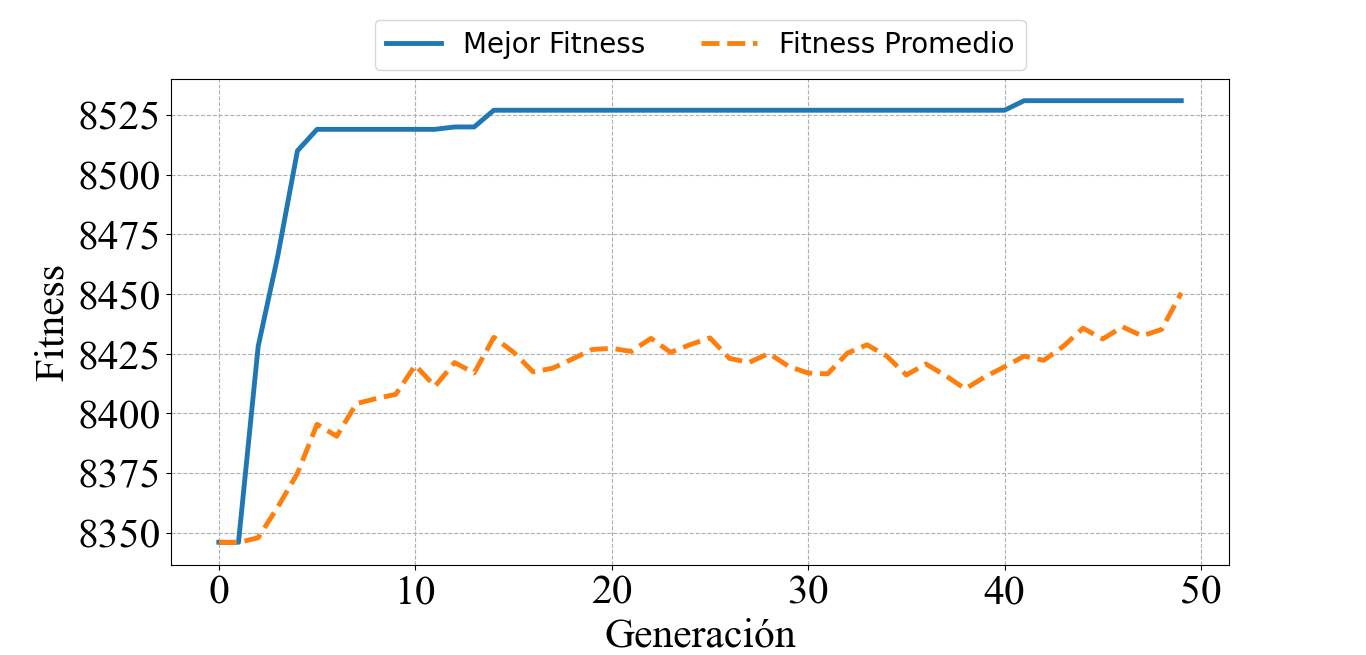
\includegraphics[width=0.9 \linewidth]{Manhattan/Fitness_individual_50Gen/Fitness_1_Manh_50Gen.png}
    \caption{Fitness individual para el entrenamiento 1 de 50 generaciones aplicando la distancia Manhattan}
    \label{fig:manhattan_1_50}
\end{figure}
\begin{figure}[H]
    \centering
    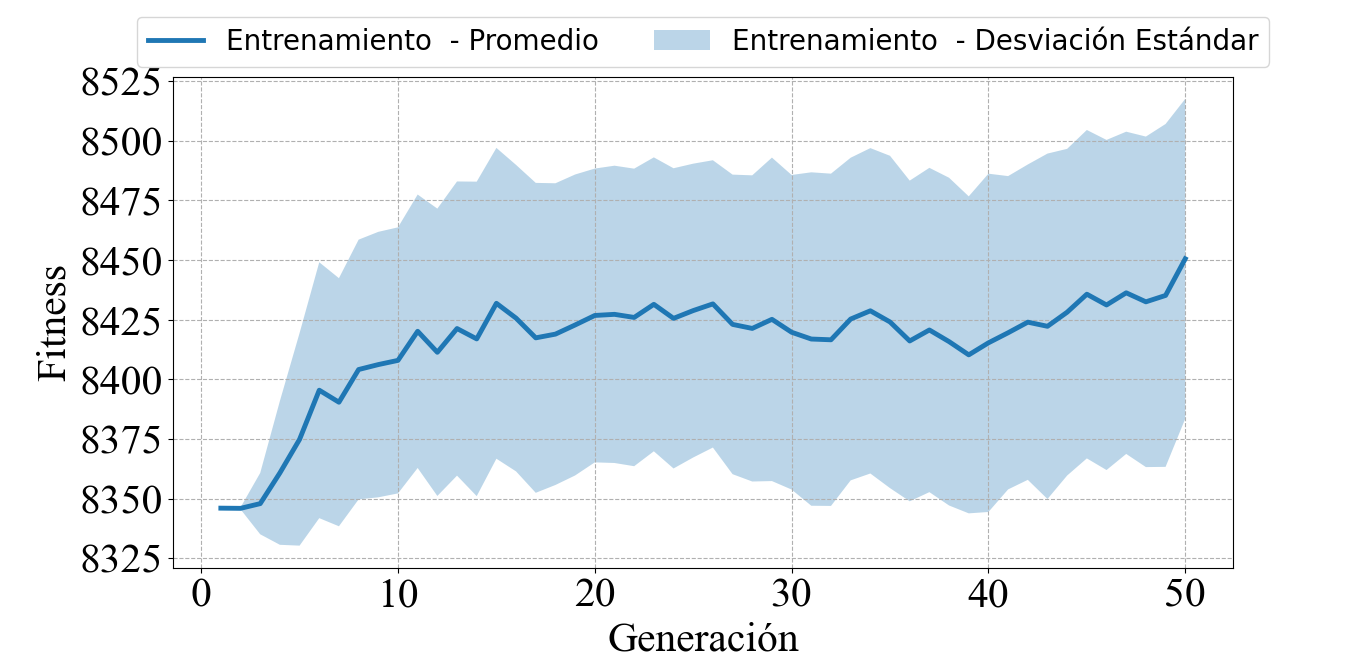
\includegraphics[width=0.9 \linewidth]{Manhattan/Fitness_individual_50Gen/Fitness_1_Manh_50Gen_Sombra.png}
    \caption{Fitness promedio y desviaciones para el entrenamiento 1 de 50 generaciones aplicando la distancia Manhattan}
    \label{fig:manhattan_1_50_sombra}
\end{figure}

\begin{figure}[H]
    \centering
    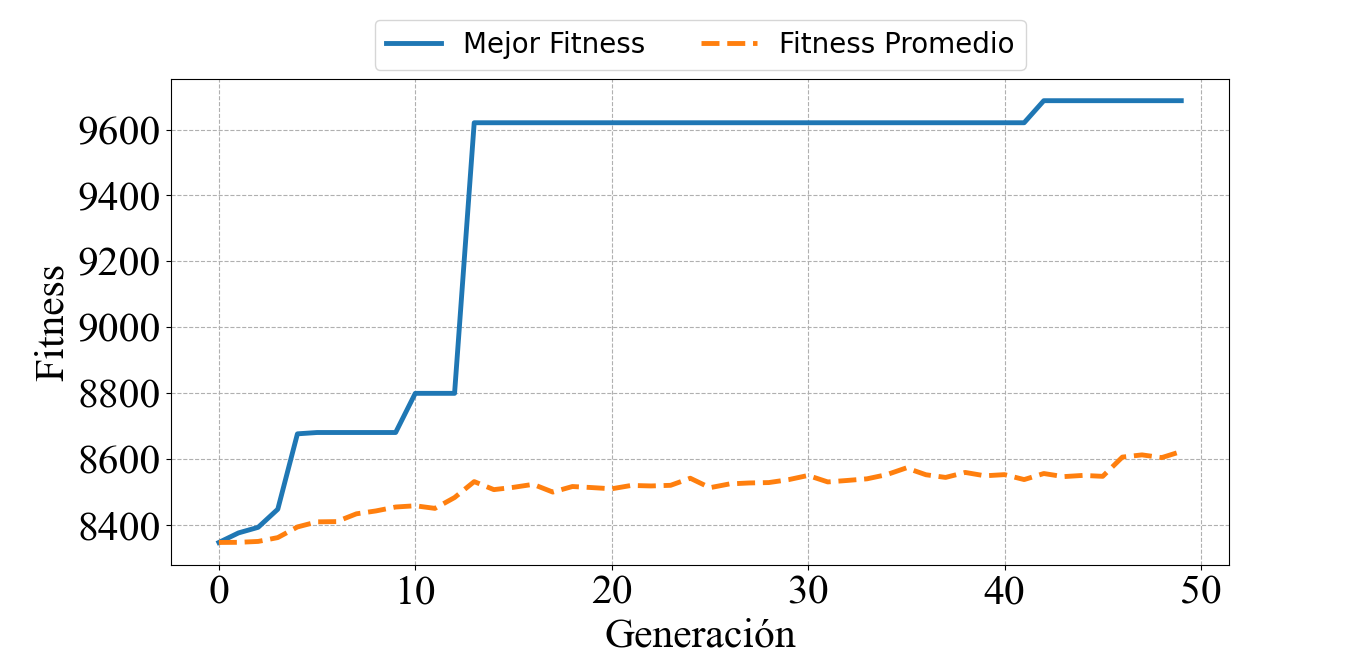
\includegraphics[width=0.9 \linewidth]{Manhattan/Fitness_individual_50Gen/Fitness_2_Manh_50Gen.png}
    \caption{Fitness individual para el entrenamiento 2 de 50 generaciones aplicando la distancia Manhattan}
    \label{fig:manhattan_2_50}
\end{figure}
\begin{figure}
    \centering
    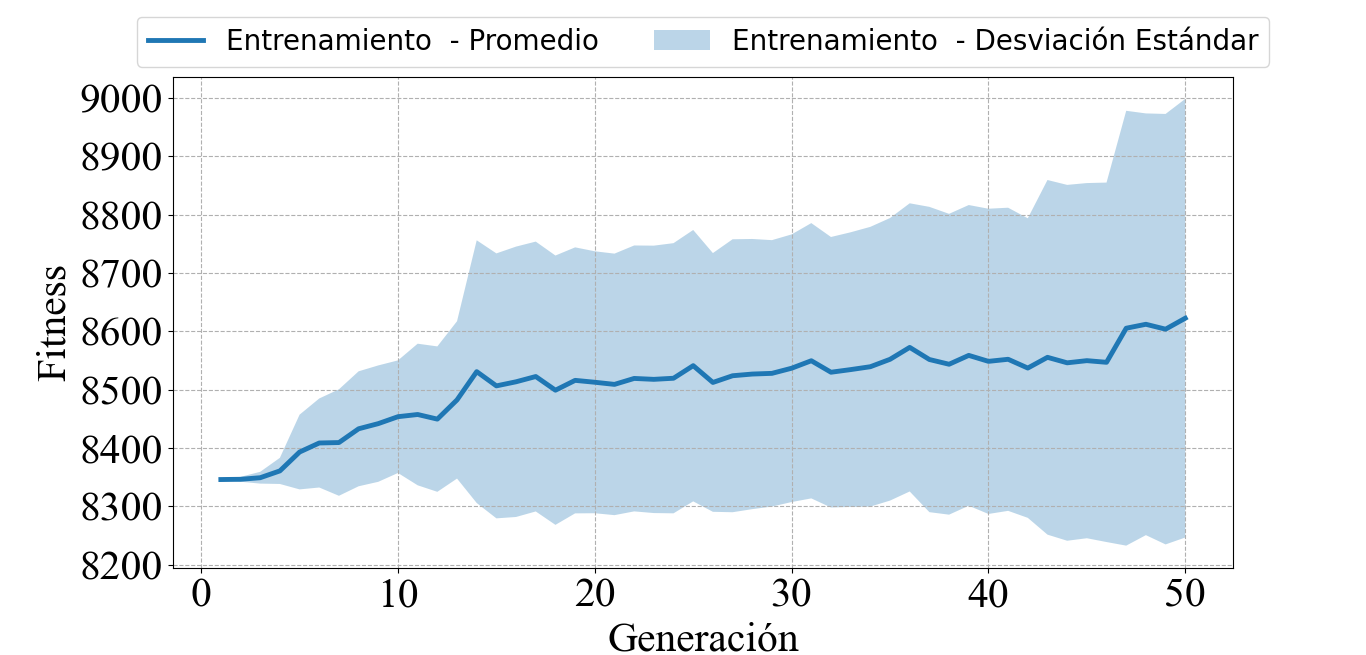
\includegraphics[width=0.9 \linewidth]{Manhattan/Fitness_individual_50Gen/Fitness_2_Manh_50Gen_Sombra.png}
    \caption{Fitness promedio y desviaciones para el entrenamiento 2 de 50 generaciones aplicando la distancia Manhattan}
    \label{fig:manhattan_2_50_sombra}
\end{figure}

\begin{figure}
    \centering
    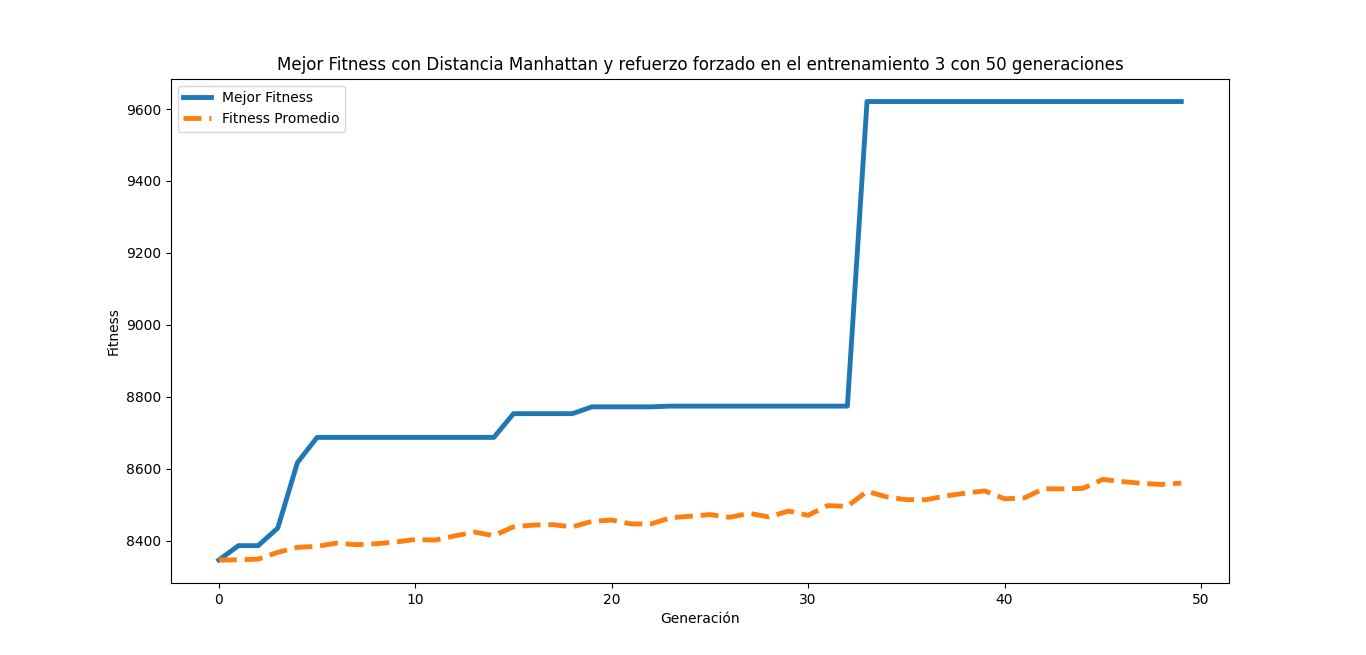
\includegraphics[width=0.9 \linewidth]{Manhattan/Fitness_individual_50Gen/Fitness_3_Manh_50Gen.png}
    \caption{Fitness individual para el entrenamiento 3 de 50 generaciones aplicando la distancia Manhattan}
    \label{fig:manhattan_3_50}
\end{figure}
\begin{figure}
    \centering
    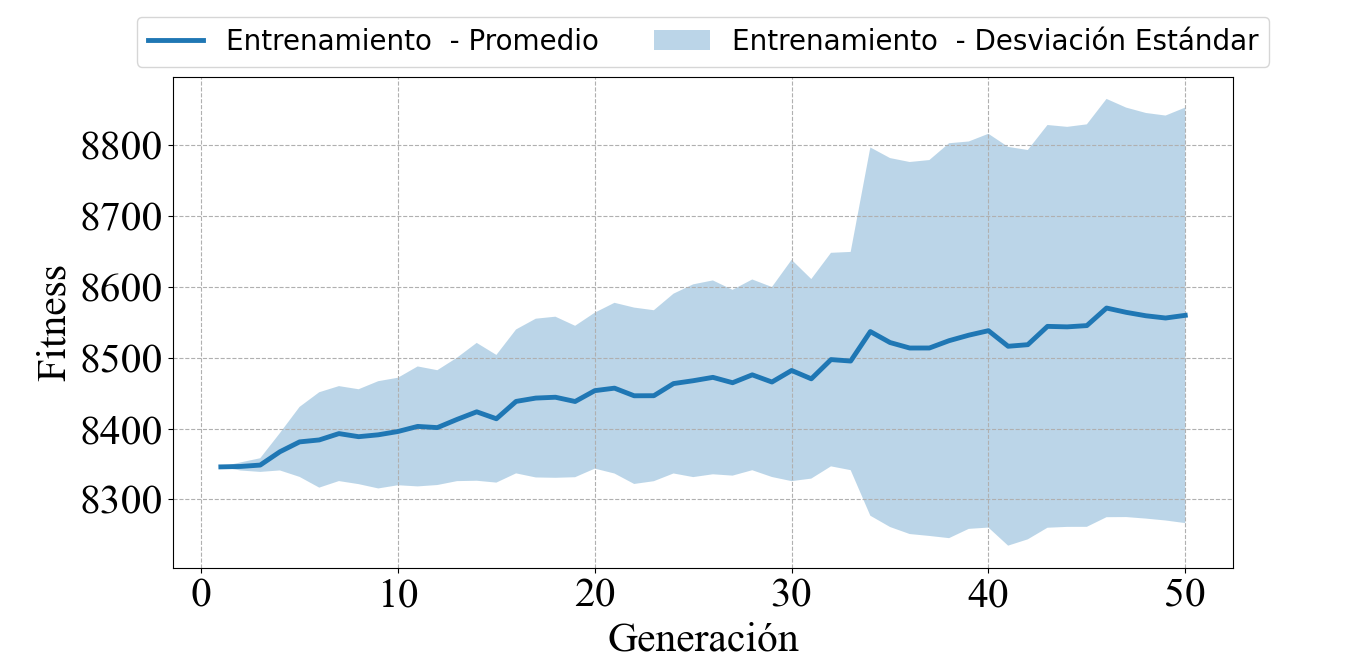
\includegraphics[width=0.9 \linewidth]{Manhattan/Fitness_individual_50Gen/Fitness_3_Manh_50Gen_Sombra.png} 
    \caption{Fitness promedio y desviaciones para el entrenamiento 3 de 50 generaciones aplicando la distancia Manhattan}
    \label{fig:manhattan_3_50_sombra}
\end{figure}

\begin{figure}
    \centering
    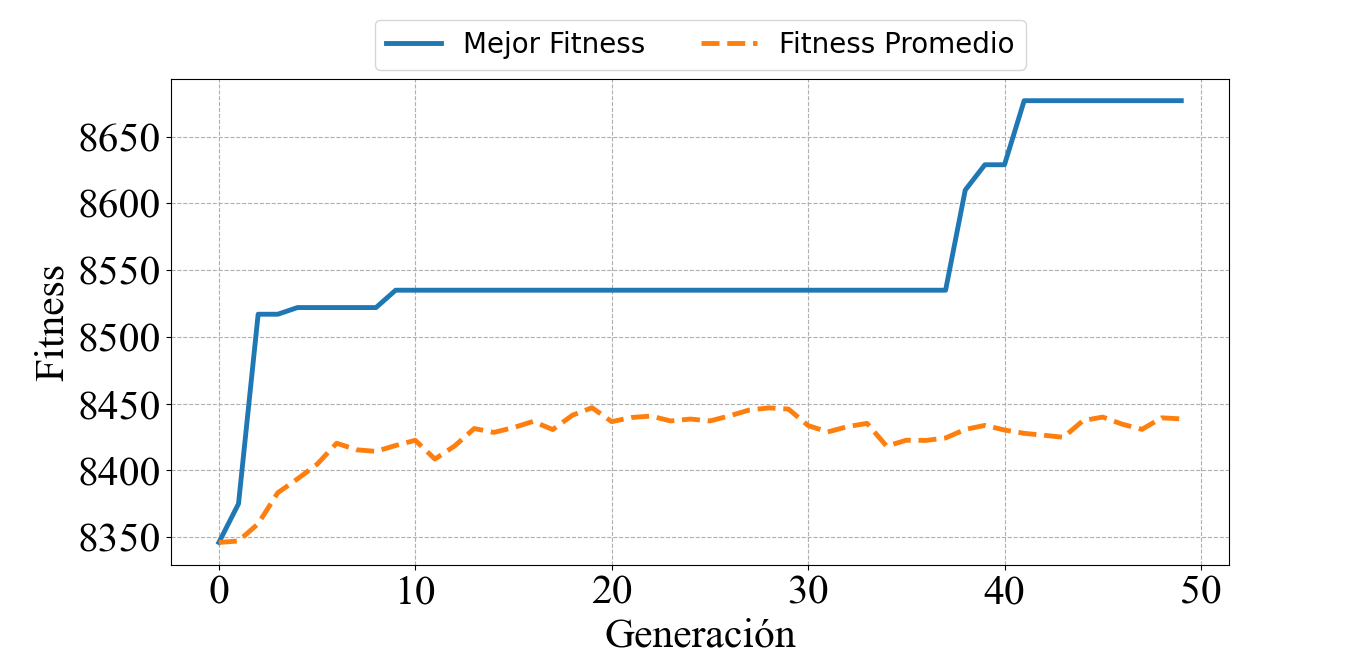
\includegraphics[width=0.9 \linewidth]{Manhattan/Fitness_individual_50Gen/Fitness_5_Manh_50Gen.png}
    \caption{Fitness individual para el entrenamiento 5 de 50 generaciones aplicando la distancia Manhattan}
    \label{fig:manhattan_5_50}
\end{figure}
\begin{figure}
    \centering
    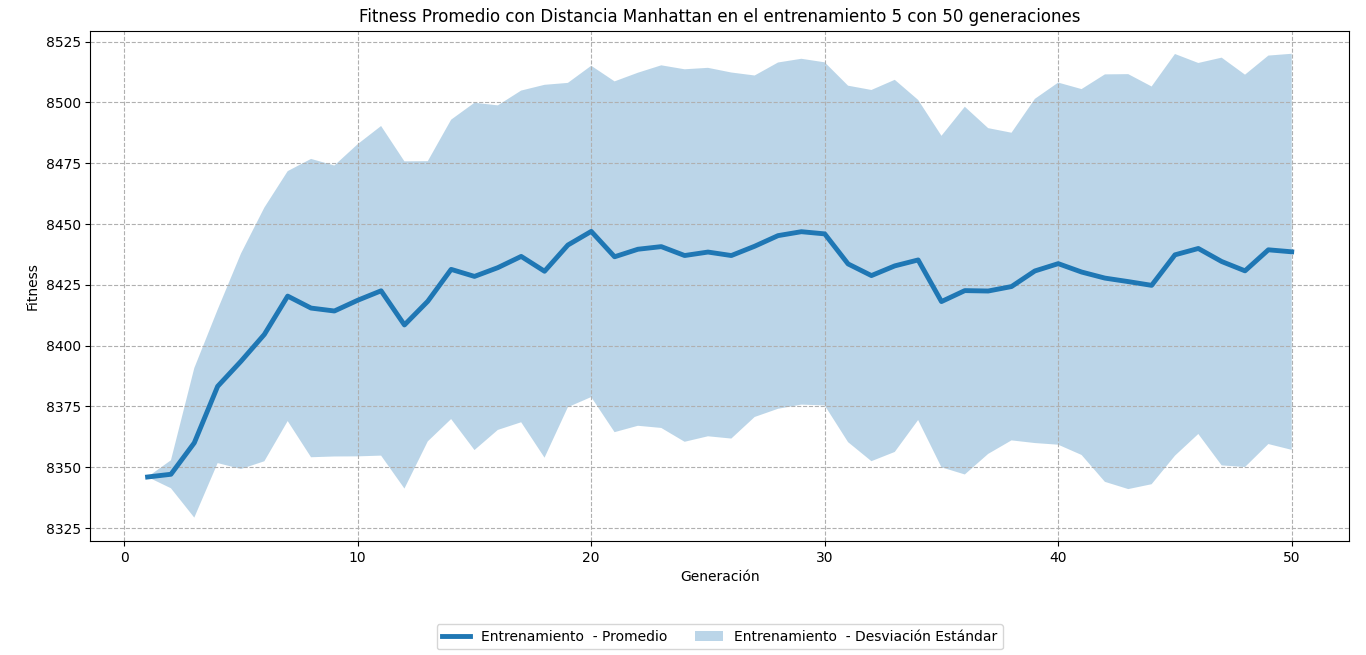
\includegraphics[width=0.9 \linewidth]{Manhattan/Fitness_individual_50Gen/Fitness_5_Manh_50Gen_Sombra.png}
    \caption{Fitness promedio y desviaciones para el entrenamiento 5 de 50 generaciones aplicando la distancia Manhattan}
    \label{fig:manhattan_5_50_sombra}
\end{figure}

\subsection{Generación 30}
\setcounter{figure}{0}
\renewcommand{\thefigure}{S\arabic{figure}B-M}

\begin{figure}[H]
    \centering
    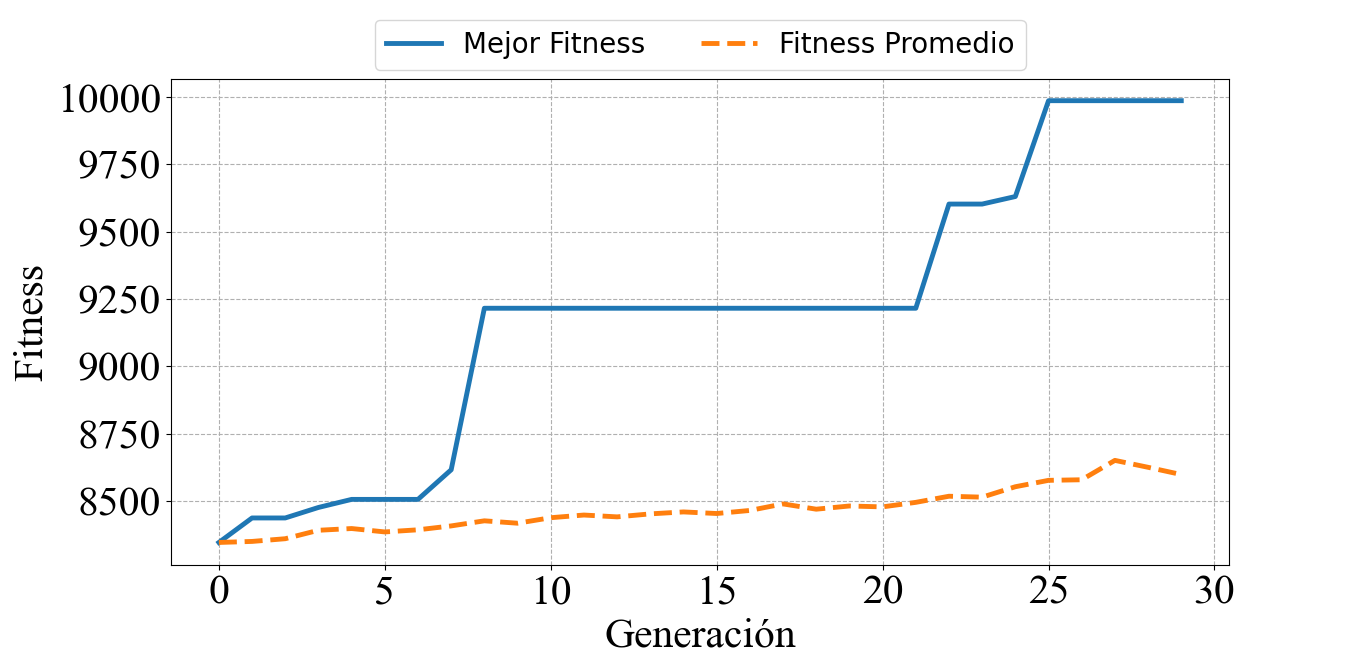
\includegraphics[width=0.9 \linewidth]{Manhattan/Fitness_individual_30Gen/Fitness_2_Mahn_30Gen.png}
    \caption{Fitness individual para el entrenamiento 2 de 30 generaciones aplicando la distancia Manhattan}
    \label{fig:manhattan_2_30}
\end{figure}
\begin{figure}[H]
    \centering
    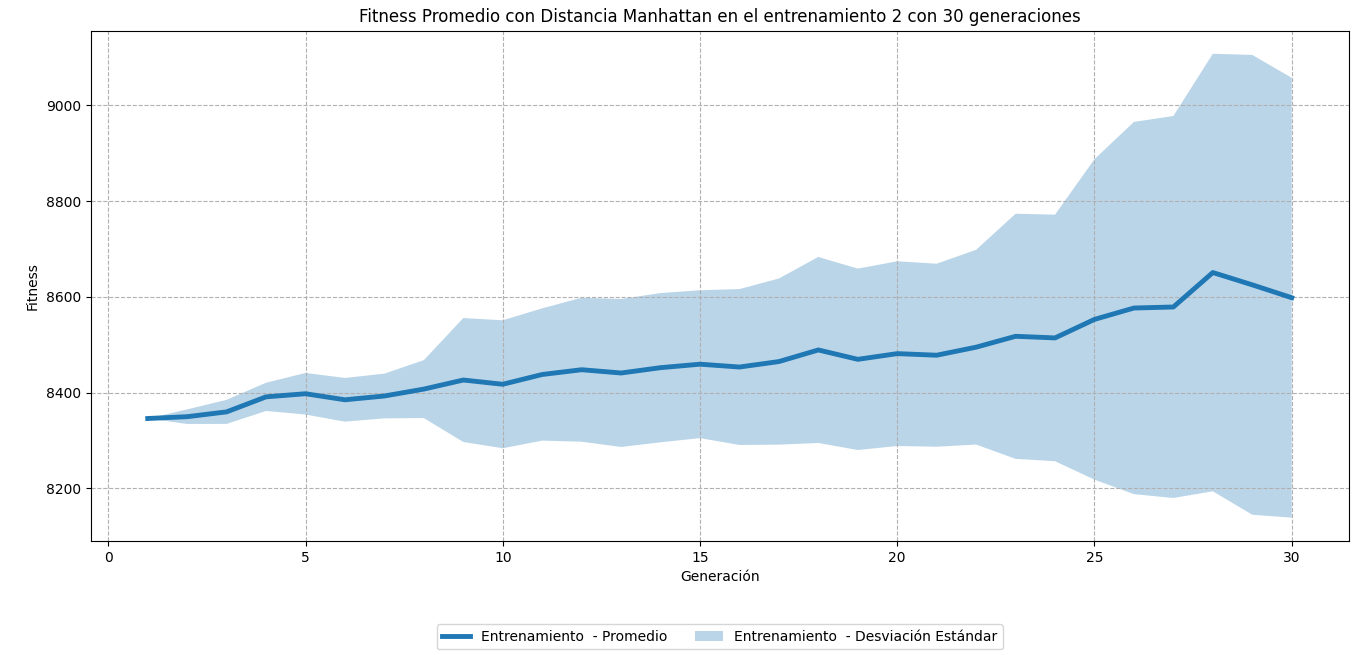
\includegraphics[width=0.9 \linewidth]{Manhattan/Fitness_individual_30Gen/Fitness_2_Mahn_30Gen_Sombra.png}
    \caption{Fitness promedio y desviaciones para el entrenamiento 2 de 30 generaciones aplicando la distancia Manhattan}
    \label{fig:manhattan_2_30_sombra}
\end{figure}

\begin{figure}[H]
    \centering
    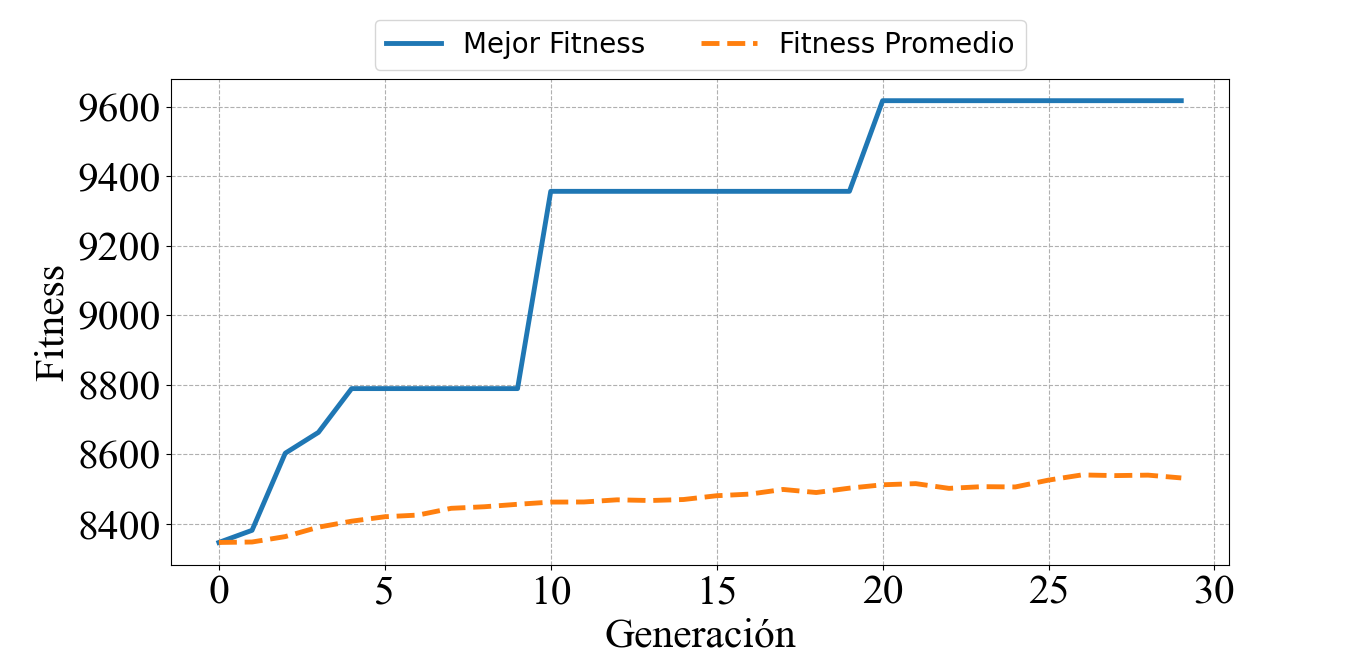
\includegraphics[width=0.9 \linewidth]{Manhattan/Fitness_individual_30Gen/Fitness_3_Mahn_30Gen.png}
    \caption{Fitness individual para el entrenamiento 3 de 30 generaciones aplicando la distancia Manhattan}
    \label{fig:manhattan_3_30}
\end{figure}
\begin{figure}[H]
    \centering
    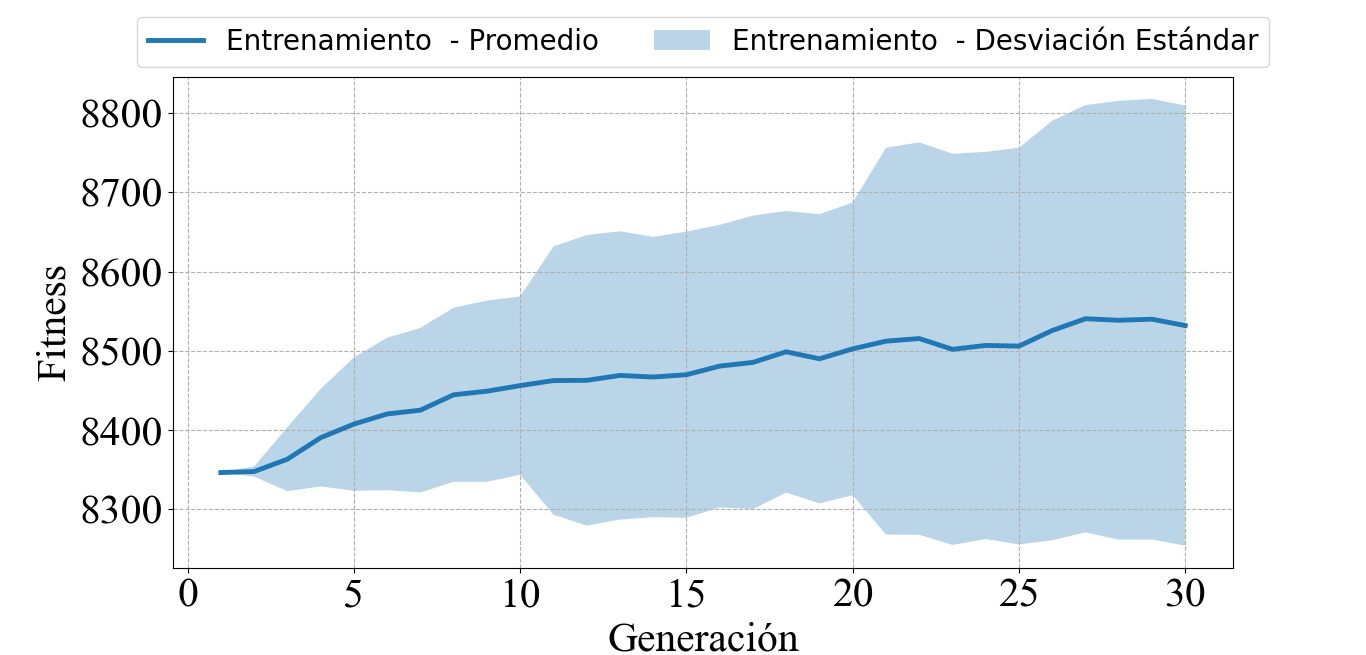
\includegraphics[width=0.9 \linewidth]{Manhattan/Fitness_individual_30Gen/Fitness_3_Mahn_30Gen_Sombra.png}
    \caption{Fitness promedio y desviaciones para el entrenamiento 3 de 30 generaciones aplicando la distancia Manhattan}
    \label{fig:manhattan_3_30_sombra}
\end{figure}

\begin{figure}[H]
    \centering
    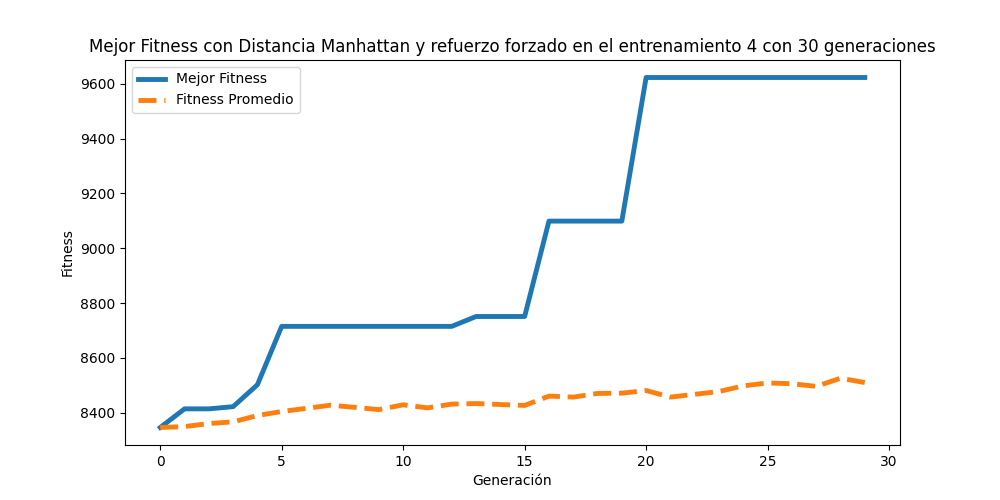
\includegraphics[width=0.9 \linewidth]{Manhattan/Fitness_individual_30Gen/Fitness_4_Mahn_30Gen.png}
    \caption{Fitness individual para el entrenamiento 4 de 30 generaciones aplicando la distancia Manhattan}
    \label{fig:manhattan_4_30}
\end{figure}

\begin{figure}[H]
    \centering
    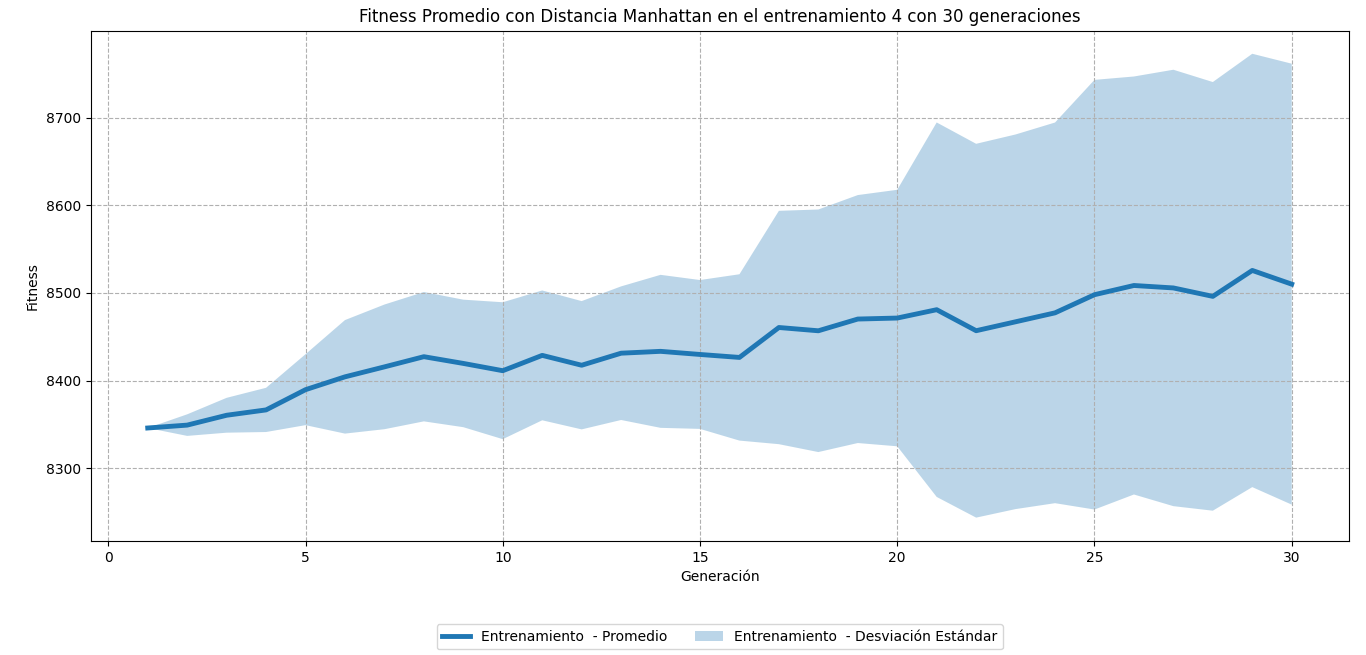
\includegraphics[width=0.9 \linewidth]{Manhattan/Fitness_individual_30Gen/Fitness_4_Mahn_30Gen_Sombra.png}
    \caption{Fitness promedio y desviaciones para el entrenamiento 4 de 30 generaciones aplicando la distancia Manhattan}
    \label{fig:manhattan_4_30_sombra}
\end{figure}
\begin{figure}[H]
    \centering
    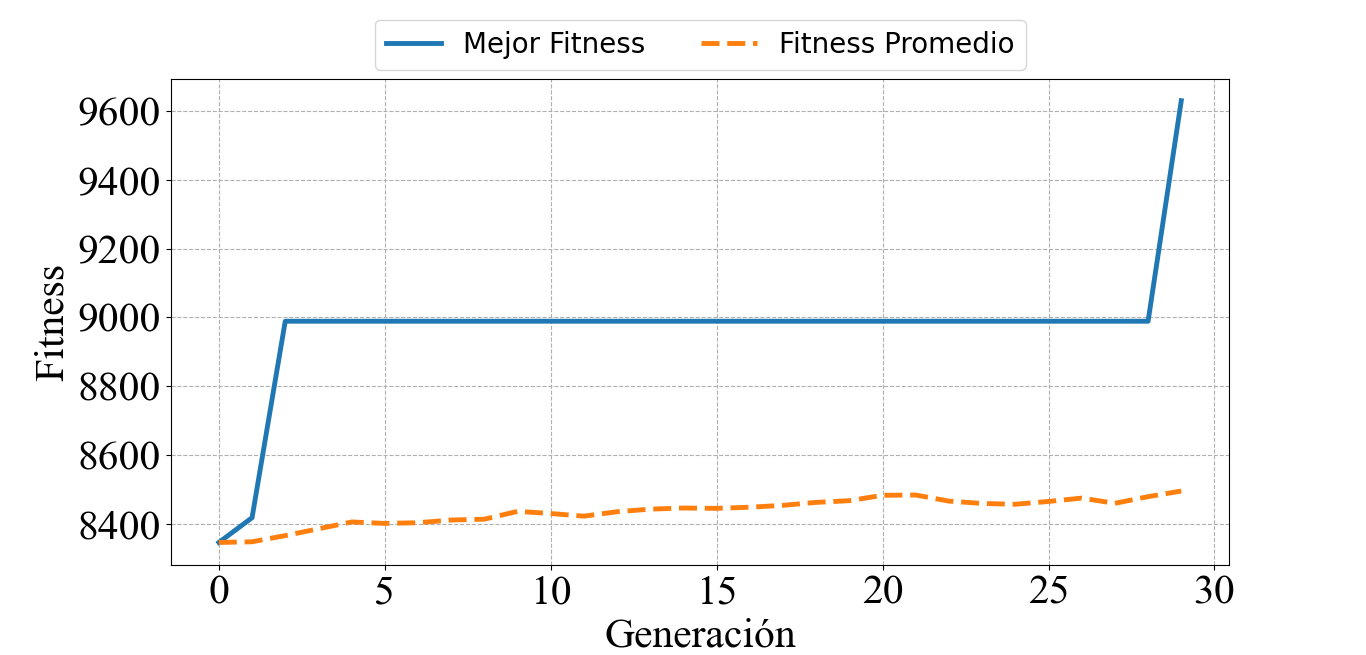
\includegraphics[width=0.9 \linewidth]{Manhattan/Fitness_individual_30Gen/Fitness_5_Mahn_30Gen.png}
    \caption{Fitness individual para el entrenamiento 5 de 30 generaciones aplicando la distancia Manhattan}
    \label{fig:manhattan_5_30}
\end{figure}

\subsection{Generación 20}
\setcounter{figure}{0}
\renewcommand{\thefigure}{S\arabic{figure}C-M}

\begin{figure}[H]
    \centering
    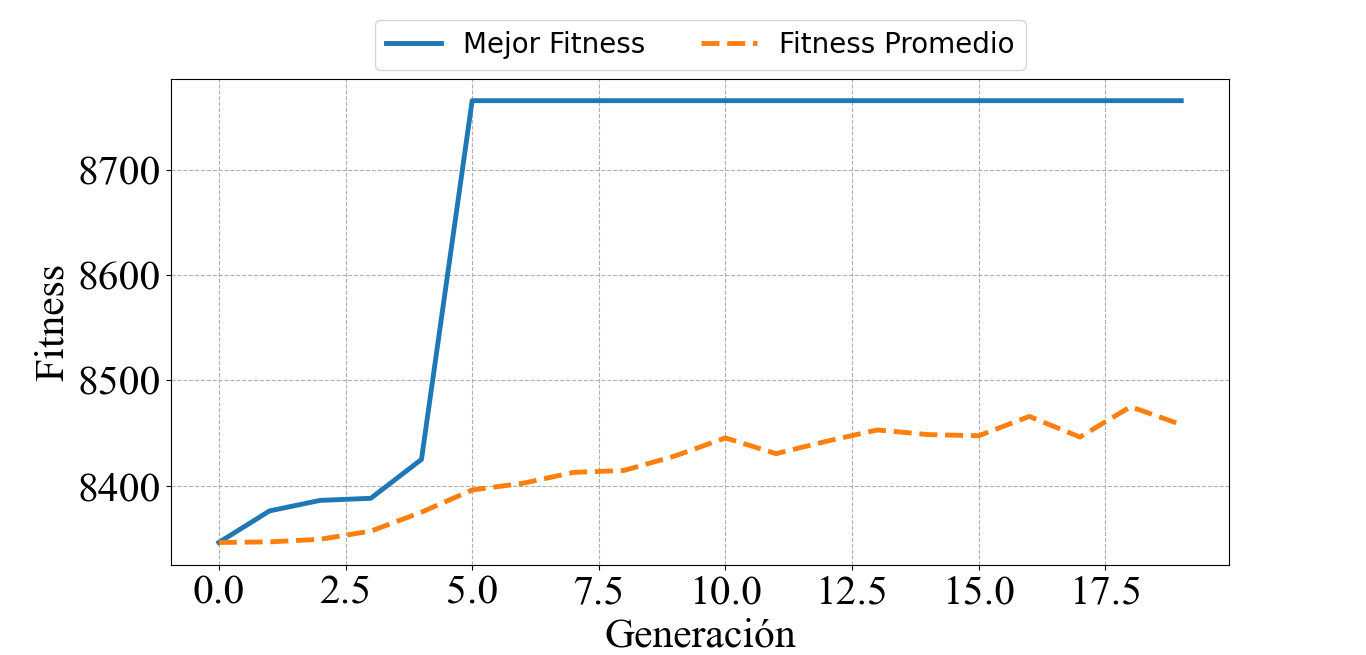
\includegraphics[width=0.9 \linewidth]{Manhattan/Fitness_individual_20Gen/Fitness_1_Manh_20Gen.png}
    \caption{Fitness individual para el entrenamiento 1 de 20 generaciones aplicando la distancia Manhattan}
    \label{fig:manhattan_1_20}
\end{figure}
\begin{figure}[H]
    \centering
    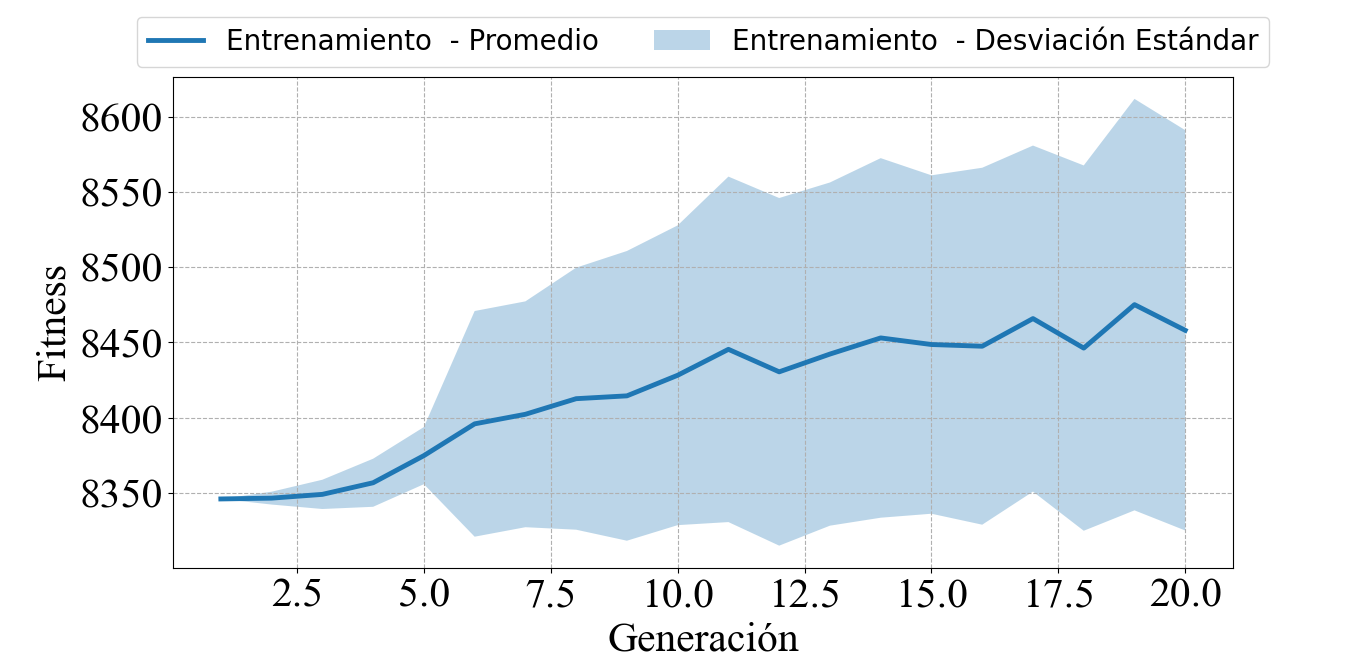
\includegraphics[width=0.9 \linewidth]{Manhattan/Fitness_individual_20Gen/Fitness_1_Manh_20Gen_Sombra.png}
    \caption{Fitness promedio y desviaciones para el entrenamiento 1 de 20 generaciones aplicando la distancia Manhattan}
    \label{fig:manhattan_1_20_sombra}
\end{figure}

\begin{figure}[H]
    \centering
    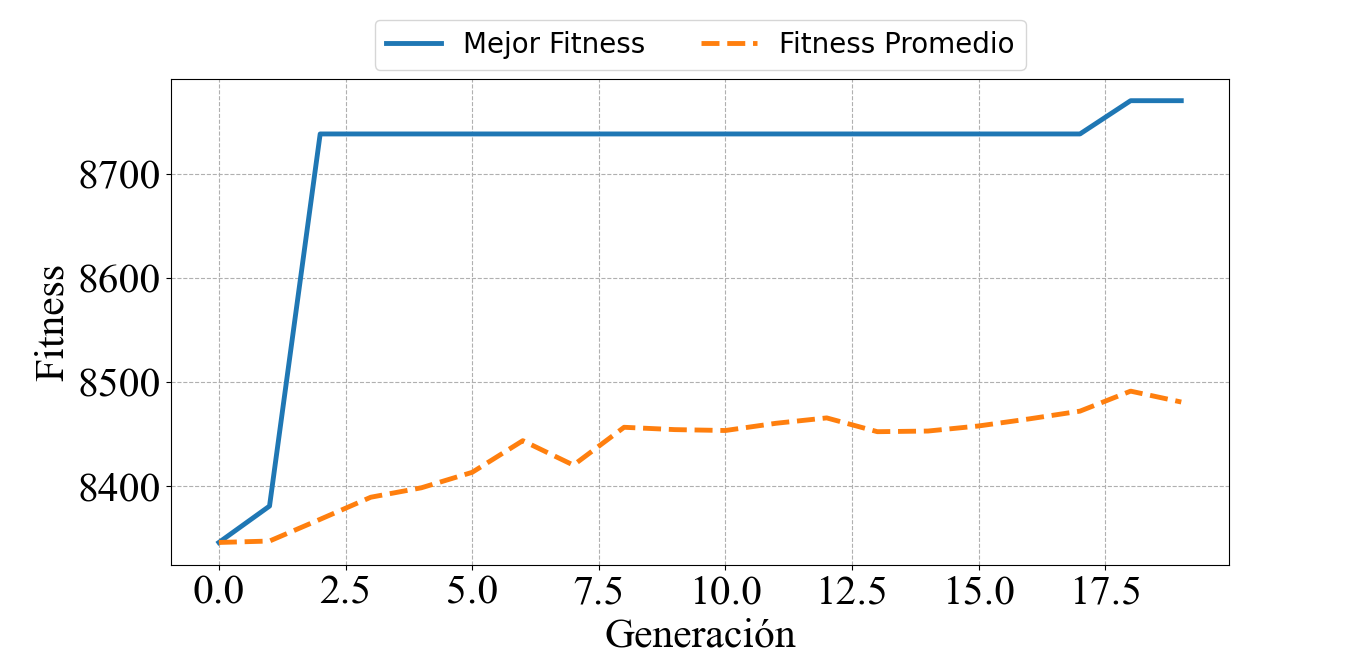
\includegraphics[width=0.9 \linewidth]{Manhattan/Fitness_individual_20Gen/Fitness_3_Manh_20Gen.png}
    \caption{Fitness individual para el entrenamiento 3 de 20 generaciones aplicando la distancia Manhattan}
    \label{fig:manhattan_3_20}
\end{figure}
\begin{figure}[H]
    \centering
    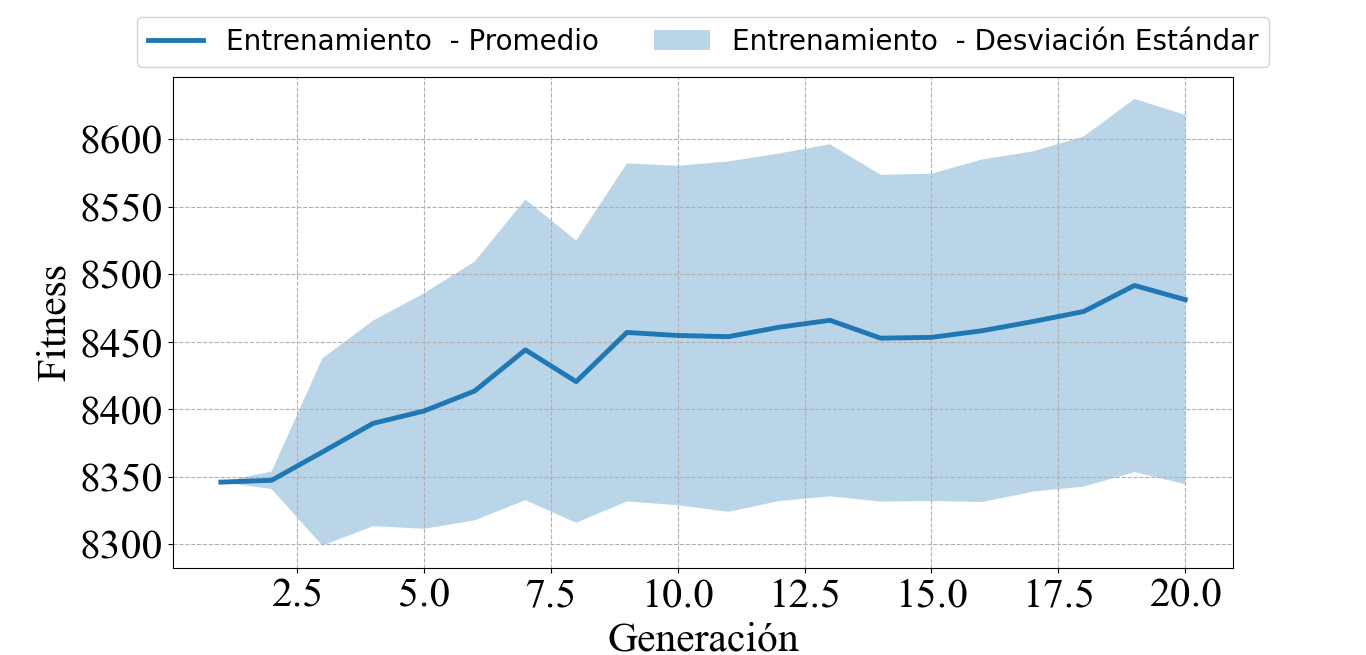
\includegraphics[width=0.9 \linewidth]{Manhattan/Fitness_individual_20Gen/Fitness_3_Manh_20Gen_Sombra.png}
    \caption{Fitness promedio y desviaciones para el entrenamiento 3 de 20 generaciones aplicando la distancia Manhattan}
    \label{fig:manhattan_3_20_sombra}
\end{figure}

\begin{figure}[H]
    \centering
    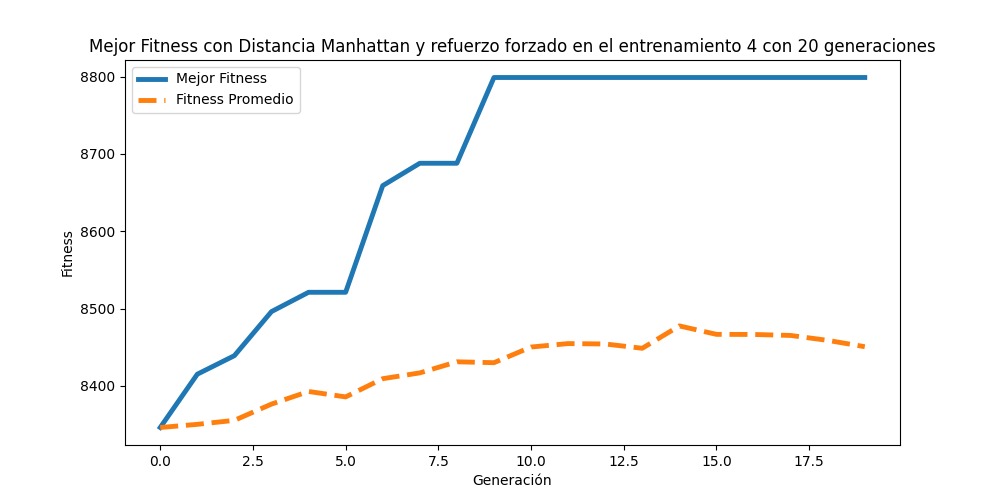
\includegraphics[width=0.9 \linewidth]{Manhattan/Fitness_individual_20Gen/Fitness_4_Manh_20Gen.png}
    \caption{Fitness individual para el entrenamiento 4 de 20 generaciones aplicando la distancia Manhattan}
    \label{fig:manhattan_4_20}
\end{figure}
\begin{figure}[H]
    \centering
    \includegraphics[width=0.9 \linewidth]{Manhattan/Fitness_individual_20Gen/Fitness_4_Manh_20Gen_Sombra.png}
    \caption{Fitness promedio y desviaciones para el entrenamiento 4 de 20 generaciones aplicando la distancia Manhattan}
    \label{fig:manhattan_4_20_sombra}
\end{figure}

\begin{figure}[H]
    \centering
    \includegraphics[width=0.9 \linewidth]{Manhattan/Fitness_individual_20Gen/Fitness_5_Manh_20Gen.png}
    \caption{Fitness individual para el entrenamiento 5 de 20 generaciones aplicando la distancia Manhattan}
    \label{fig:manhattan_5_20}
\end{figure}
\begin{figure}[H]
    \centering
    \includegraphics[width=0.9 \linewidth]{Manhattan/Fitness_individual_20Gen/Fitness_5_Manh_20Gen_Sombra.png}
    \caption{Fitness promedio y desviaciones para el entrenamiento 5 de 20 generaciones aplicando la distancia Manhattan}
    \label{fig:manhattan_5_20_sombra}
\end{figure}

\section{Resultados de las simulaciones para la distancia Chebyshev}
\subsection{Generación 50}
\setcounter{figure}{0}
\renewcommand{\thefigure}{S\arabic{figure}A-C}
\begin{figure}[H]
    \centering
    \includegraphics[width=0.9 \linewidth]{Chebyshev/Fitness_individual_50Gen/Fitness_1_Cheby_50Gen.png}
    \caption{Fitness individual para el entrenamiento 1 de 50 generaciones aplicando la distancia Chebyshev}
    \label{fig:cheb_1_50}
\end{figure}
\begin{figure}[H]
    \centering
    \includegraphics[width=0.9 \linewidth]{Chebyshev/Fitness_individual_50Gen/Fitness_1_Cheby_50Gen_Sombra.png}
    \caption{Fitness promedio y desviaciones para el entrenamiento 1 de 50 generaciones aplicando la distancia Chebyshev}
    \label{fig:cheb_1_50_sombra}
\end{figure}

\begin{figure}[H]
    \centering
    \includegraphics[width=0.9 \linewidth]{Chebyshev/Fitness_individual_50Gen/Fitness_2_Cheby_50Gen.png}
    \caption{Fitness individual para el entrenamiento 2 de 50 generaciones aplicando la distancia Chebyshev}
    \label{fig:cheb_2_50}
\end{figure}
\begin{figure}[H]
    \centering
    \includegraphics[width=0.9 \linewidth]{Chebyshev/Fitness_individual_50Gen/Fitness_2_Cheby_50Gen_Sombra.png}
    \caption{Fitness promedio y desviaciones para el entrenamiento 2 de 50 generaciones aplicando la distancia Chebyshev}
    \label{fig:cheb_2_50_sombra}
\end{figure}

\begin{figure}[H]
    \centering
    \includegraphics[width=0.9 \linewidth]{Chebyshev/Fitness_individual_50Gen/Fitness_3_Cheby_50Gen.png}
    \caption{Fitness individual para el entrenamiento 3 de 50 generaciones aplicando la distancia Chebyshev}
    \label{fig:cheb_3_50}
\end{figure}
\begin{figure}[H]
    \centering
    \includegraphics[width=0.9 \linewidth]{Chebyshev/Fitness_individual_50Gen/Fitness_3_Cheby_50Gen_Sombra.png}
    \caption{Fitness promedio y desviaciones para el entrenamiento 3 de 50 generaciones aplicando la distancia Chebyshev}
    \label{fig:cheb_3_50_sombra}
\end{figure}

\begin{figure}[H]
    \centering
    \includegraphics[width=0.9 \linewidth]{Chebyshev/Fitness_individual_50Gen/Fitness_4_Cheby_50Gen.png}
    \caption{Fitness individual para el entrenamiento 4 de 50 generaciones aplicando la distancia Chebyshev}
    \label{fig:cheb_4_50}
\end{figure}
\begin{figure}[H]
    \centering
    \includegraphics[width=0.9 \linewidth]{Chebyshev/Fitness_individual_50Gen/Fitness_4_Cheby_50Gen_Sombra.png}
    \caption{Fitness promedio y desviaciones para el entrenamiento 4 de 50 generaciones aplicando la distancia Chebyshev}
    \label{fig:cheb_4_50_sombra}
\end{figure}

\begin{figure}[H]
    \centering
    \includegraphics[width=0.9 \linewidth]{Chebyshev/Fitness_individual_50Gen/Fitness_5_Cheby_50Gen.png}
    \caption{Fitness individual para el entrenamiento 5 de 50 generaciones aplicando la distancia Chebyshev}
    \label{fig:cheb_5_50}
\end{figure}
\begin{figure}[H]
    \centering
    \includegraphics[width=0.9 \linewidth]{Chebyshev/Fitness_individual_50Gen/Fitness_5_Cheby_50Gen_Sombra.png}
    \caption{Fitness promedio y desviaciones para el entrenamiento 5 de 50 generaciones aplicando la distancia Chebyshev}
    \label{fig:cheb_5_50_sombra}
\end{figure}

\subsection{Generación 30}
\setcounter{figure}{0}
\renewcommand{\thefigure}{S\arabic{figure}B-C}

\begin{figure}[H]
    \centering
    \includegraphics[width=0.9 \linewidth]{Chebyshev/Fitness_individual_30Gen/Fitness_1_Cheby_30Gen.png}
    \caption{Fitness individual para el entrenamiento 1 de 30 generaciones aplicando la distancia Chebyshev}
    \label{fig:cheb_1_30}
\end{figure}
\begin{figure}[H]
    \centering
    \includegraphics[width=0.9 \linewidth]{Chebyshev/Fitness_individual_30Gen/Fitness_1_Cheby_30Gen_Sombra.png}
    \caption{Fitness promedio y desviaciones para el entrenamiento 1 de 30 generaciones aplicando la distancia Chebyshev}
    \label{fig:cheb_1_30_sombra}
\end{figure}

\begin{figure}[H]
    \centering
    \includegraphics[width=0.9 \linewidth]{Chebyshev/Fitness_individual_30Gen/Fitness_2_Cheby_30Gen_Sombra.png}
    \caption{Fitness individual para el entrenamiento 2 de 30 generaciones aplicando la distancia Chebyshev}
    \label{fig:cheb_2_30_sombra}
\end{figure}



\begin{figure}[H]
    \centering
    \includegraphics[width=0.9 \linewidth]{Chebyshev/Fitness_individual_30Gen/Fitness_3_Cheby_30Gen.png}
    \caption{Fitness individual para el entrenamiento 3 de 30 generaciones aplicando la distancia Chebyshev}
    \label{fig:cheb_3_30}
\end{figure}
\begin{figure}[H]
    \centering
    \includegraphics[width=0.9 \linewidth]{Chebyshev/Fitness_individual_30Gen/Fitness_3_Cheby_30Gen_Sombra.png}
    \caption{Fitness promedio y desviaciones para el entrenamiento 3 de 30 generaciones aplicando la distancia Chebyshev}
    \label{fig:cheb_3_30_sombra}
\end{figure}

\begin{figure}[H]
    \centering
    \includegraphics[width=0.9 \linewidth]{Chebyshev/Fitness_individual_30Gen/Fitness_4_Cheby_30Gen.png}
    \caption{Fitness individual para el entrenamiento 4 de 30 generaciones aplicando la distancia Chebyshev}
    \label{fig:cheb_4_30}
\end{figure}
\begin{figure}[H]
    \centering
    \includegraphics[width=0.9 \linewidth]{Chebyshev/Fitness_individual_30Gen/Fitness_4_Cheby_30Gen_Sombra.png}
    \caption{Fitness promedio y desviaciones para el entrenamiento 4 de 30 generaciones aplicando la distancia Chebyshev}
    \label{fig:cheb_4_30_sombra}
\end{figure}

\begin{figure}[H]
    \centering
    \includegraphics[width=0.9 \linewidth]{Chebyshev/Fitness_individual_30Gen/Fitness_5_Cheby_30Gen.png}
    \caption{Fitness individual para el entrenamiento 5 de 30 generaciones aplicando la distancia Chebyshev}
    \label{fig:cheb_5_30}
\end{figure}
\begin{figure}[H]
    \centering
    \includegraphics[width=0.9 \linewidth]{Chebyshev/Fitness_individual_30Gen/Fitness_5_Cheby_30Gen_Sombra.png}
    \caption{Fitness promedio y desviaciones para el entrenamiento 5 de 30 generaciones aplicando la distancia Chebyshev}
    \label{fig:cheb_5_30_sombra}
\end{figure}


\subsection{Generación 20}
\setcounter{figure}{0}
\renewcommand{\thefigure}{S\arabic{figure}C-C}

\begin{figure}[H]
    \centering
    \includegraphics[width=0.9 \linewidth]{Chebyshev/Fitness_individual_20Gen/Fitness_1_Cheby_20Gen.png}
    \caption{Fitness individual para el entrenamiento 1 de 20 generaciones aplicando la distancia Chebyshev}
    \label{fig:cheb_1_20}
\end{figure}
\begin{figure}[H]
    \centering
    \includegraphics[width=0.9 \linewidth]{Chebyshev/Fitness_individual_20Gen/Fitness_1_Cheby_20Gen_Sombra.png}
    \caption{Fitness promedio y desviaciones para el entrenamiento 1 de 20 generaciones aplicando la distancia Chebyshev}
    \label{fig:cheb_1_20_sombra}
\end{figure}

\begin{figure}[H]
    \centering
    \includegraphics[width=0.9 \linewidth]{Chebyshev/Fitness_individual_20Gen/Fitness_3_Cheby_20Gen.png}
    \caption{Fitness individual para el entrenamiento 3 de 20 generaciones aplicando la distancia Chebyshev}
    \label{fig:cheb_3_20}
\end{figure}
\begin{figure}[H]
    \centering
    \includegraphics[width=0.9 \linewidth]{Chebyshev/Fitness_individual_20Gen/Fitness_3_Cheby_20Gen_Sombra.png}
    \caption{Fitness promedio y desviaciones para el entrenamiento 3 de 20 generaciones aplicando la distancia Chebyshev}
    \label{fig:cheb_3_20_sombra}
\end{figure}

\begin{figure}[H]
    \centering
    \includegraphics[width=0.9 \linewidth]{Chebyshev/Fitness_individual_20Gen/Fitness_4_Cheby_20Gen.png}
    \caption{Fitness individual para el entrenamiento 4 de 20 generaciones aplicando la distancia Chebyshev}
    \label{fig:cheb_4_20}
\end{figure}
\begin{figure}[H]
    \centering
    \includegraphics[width=0.9 \linewidth]{Chebyshev/Fitness_individual_20Gen/Fitness_4_Cheby_20Gen_Sombra.png}
    \caption{Fitness promedio y desviaciones para el entrenamiento 4 de 20 generaciones aplicando la distancia Chebyshev}
    \label{fig:cheb_4_20_sombra}
\end{figure}

\begin{figure}[H]
    \centering
    \includegraphics[width=0.9 \linewidth]{Chebyshev/Fitness_individual_20Gen/Fitness_5_Cheby_20Gen.png}
    \caption{Fitness individual para el entrenamiento 5 de 20 generaciones aplicando la distancia Chebyshev}
    \label{fig:cheb_5_20}
\end{figure}
\begin{figure}[H]
    \centering
    \includegraphics[width=0.9 \linewidth]{Chebyshev/Fitness_individual_20Gen/Fitness_5_Cheby_20Gen_Sombra.png}
    \caption{Fitness promedio y desviaciones para el entrenamiento 5 de 20 generaciones aplicando la distancia Chebyshev}
    \label{fig:cheb_5_20_sombra}
\end{figure}


\section{Resultados de las simulaciones con el segundo mapa y Refuerzo Forzado}
\subsection{Distancia Euclidiana}
\setcounter{figure}{0}
\renewcommand{\thefigure}{S\arabic{figure}-EM2}

\begin{figure}[H]
    \centering
    \includegraphics[width=0.9 \linewidth]{Euclidiana/Mapa2/Fitness_1_Map2_Eucli_50Gen.png}
    \caption{Fitness individual para el entrenamiento 1 de 50 generaciones aplicando la distancia Euclidiana en el segundo mapa}
    \label{fig:eucli_1_50_m2}
\end{figure}
\begin{figure}[H]
    \centering
    \includegraphics[width=0.9 \linewidth]{Euclidiana/Mapa2/Fitness_1_Map2_Eucli_50Gen_Sombra.png}
    \caption{Fitness promedio y desviaciones para el entrenamiento 1 de 50 generaciones aplicando la distancia Euclidiana en el segundo mapa}
    \label{fig:eucli_1_50_sombra_m2}
\end{figure}

\begin{figure}[H]
    \centering
    \includegraphics[width=0.9 \linewidth]{Euclidiana/Mapa2/Fitness_2_Map2_Eucli_50Gen.png}
    \caption{Fitness individual para el entrenamiento 2 de 50 generaciones aplicando la distancia Euclidiana en el segundo mapa}
    \label{fig:eucli_2_50_m2}
\end{figure}
\begin{figure}[H]
    \centering
    \includegraphics[width=0.9 \linewidth]{Euclidiana/Mapa2/Fitness_2_Map2_Eucli_50Gen_Sombra.png}
    \caption{Fitness promedio y desviaciones para el entrenamiento 2 de 50 generaciones aplicando la distancia Euclidiana en el segundo mapa}
    \label{fig:eucli_2_50_sombra_m2}
\end{figure}

\begin{figure}[H]
    \centering
    \includegraphics[width=0.9 \linewidth]{Euclidiana/Mapa2/Fitness_3_Map2_Eucli_50Gen.png}
    \caption{Fitness individual para el entrenamiento 3 de 50 generaciones aplicando la distancia Euclidiana en el segundo mapa}
    \label{fig:eucli_3_50_m2}
\end{figure}
\begin{figure}[H]
    \centering
    \includegraphics[width=0.9 \linewidth]{Euclidiana/Mapa2/Fitness_3_Map2_Eucli_50Gen_Sombra.png}
    \caption{Fitness promedio y desviaciones para el entrenamiento 3 de 50 generaciones aplicando la distancia Euclidiana en el segundo mapa}
    \label{fig:eucli_3_50_sombra_m2}
\end{figure}

\begin{figure}[H]
    \centering
    \includegraphics[width=0.9 \linewidth]{Euclidiana/Mapa2/Fitness_4_Map2_Eucli_50Gen.png}
    \caption{Fitness individual para el entrenamiento 4 de 50 generaciones aplicando la distancia Euclidiana en el segundo mapa}
    \label{fig:eucli_4_50_m2}
\end{figure}
\begin{figure}[H]
    \centering
    \includegraphics[width=0.9 \linewidth]{Euclidiana/Mapa2/Fitness_4_Map2_Eucli_50Gen_Sombra.png}
    \caption{Fitness promedio y desviaciones para el entrenamiento 4 de 50 generaciones aplicando la distancia Euclidiana en el segundo mapa}
    \label{fig:eucli_4_50_sombra_m2}
\end{figure}

\begin{figure}[H]
    \centering
    \includegraphics[width=0.9 \linewidth]{Euclidiana/Mapa2/Fitness_5_Map2_Eucli_50Gen.png}
    \caption{Fitness individual para el entrenamiento 5 de 50 generaciones aplicando la distancia Euclidiana en el segundo mapa}
    \label{fig:eucli_5_50_m2}
\end{figure}
\begin{figure}[H]
    \centering
    \includegraphics[width=0.9 \linewidth]{Euclidiana/Mapa2/Fitness_5_Map2_Eucli_50Gen_Sombra.png}
    \caption{Fitness promedio y desviaciones para el entrenamiento 5 de 50 generaciones aplicando la distancia Euclidiana en el segundo mapa}
    \label{fig:eucli_5_50_sombra_m2}
\end{figure}


\subsection{Distancia Manhattan}
\setcounter{figure}{0}
\renewcommand{\thefigure}{S\arabic{figure}-MM2}

\begin{figure}[H]
    \centering
    \includegraphics[width=0.9 \linewidth]{Manhattan/Mapa2/Fitness_1_Map2_Manh_50Gen.png}
    \caption{Fitness individual para el entrenamiento 1 de 50 generaciones aplicando la distancia Manhattan en el segundo mapa}
    \label{fig:manh_1_50_m2}
\end{figure}
\begin{figure}[H]
    \centering
    \includegraphics[width=0.9 \linewidth]{Manhattan/Mapa2/Fitness_1_Map2_Manh_50Gen_Sombra.png}
    \caption{Fitness promedio y desviaciones para el entrenamiento 1 de 50 generaciones aplicando la distancia Manhattan en el segundo mapa}
    \label{fig:manh_1_50_sombra_m2}
\end{figure}

\begin{figure}[H]
    \centering
    \includegraphics[width=0.9 \linewidth]{Manhattan/Mapa2/Fitness_2_Map2_Manh_50Gen.png}
    \caption{Fitness individual para el entrenamiento 2 de 50 generaciones aplicando la distancia Manhattan en el segundo mapa}
    \label{fig:manh_2_50_m2}
\end{figure}

\begin{figure}[H]
    \centering
    \includegraphics[width=0.9 \linewidth]{Manhattan/Mapa2/Fitness_2_Map2_Manh_50Gen_Sombra.png}
    \caption{Fitness promedio y desviaciones para el entrenamiento 2 de 50 generaciones aplicando la distancia Manhattan en el segundo mapa}
    \label{fig:manh_2_50_sombra_m2}
\end{figure}

\begin{figure}[H]
    \centering
    \includegraphics[width=0.9 \linewidth]{Manhattan/Mapa2/Fitness_3_Map2_Manh_50Gen.png}
    \caption{Fitness individual para el entrenamiento 3 de 50 generaciones aplicando la distancia Manhattan en el segundo mapa}
    \label{fig:manh_3_50_m2}
\end{figure}
\begin{figure}[H]
    \centering
    \includegraphics[width=0.9 \linewidth]{Manhattan/Mapa2/Fitness_3_Map2_Manh_50Gen_Sombra.png}
    \caption{Fitness promedio y desviaciones para el entrenamiento 3 de 50 generaciones aplicando la distancia Manhattan en el segundo mapa}
    \label{fig:manh_3_50_sombra_m2}
\end{figure}

\begin{figure}[H]
    \centering
    \includegraphics[width=0.9 \linewidth]{Manhattan/Mapa2/Fitness_4_Map2_Manh_50Gen.png}
    \caption{Fitness individual para el entrenamiento 4 de 50 generaciones aplicando la distancia Manhattan en el segundo mapa}
    \label{fig:manh_4_50_m2}
\end{figure}
\begin{figure}[H]
    \centering
    \includegraphics[width=0.9 \linewidth]{Manhattan/Mapa2/Fitness_4_Map2_Manh_50Gen_Sombra.png}
    \caption{Fitness promedio y desviaciones para el entrenamiento 4 de 50 generaciones aplicando la distancia Manhattan en el segundo mapa}
    \label{fig:manh_4_50_sombra_m2}
\end{figure}

\begin{figure}[H]
    \centering
    \includegraphics[width=0.9 \linewidth]{Manhattan/Mapa2/Fitness_5_Map2_Manh_50Gen.png}
    \caption{Fitness individual para el entrenamiento 5 de 50 generaciones aplicando la distancia Manhattan en el segundo mapa}
    \label{fig:manh_5_50_m2}
\end{figure}
\begin{figure}[H]
    \centering
    \includegraphics[width=0.9 \linewidth]{Manhattan/Mapa2/Fitness_5_Map2_Manh_50Gen_Sombra.png}
    \caption{Fitness promedio y desviaciones para el entrenamiento 5 de 50 generaciones aplicando la distancia Manhattan en el segundo mapa}
    \label{fig:manh_5_50_sombra_m2}
\end{figure}

\subsection{Distancia Chebyshev}
\setcounter{figure}{0}
\renewcommand{\thefigure}{S\arabic{figure}-CM2}

\begin{figure}[H]
    \centering
    \includegraphics[width=0.9 \linewidth]{Chebyshev/Mapa2/Fitness_1_Map2_Cheby_50Gen.png}
    \caption{Fitness individual para el entrenamiento 1 de 50 generaciones aplicando la distancia Chebyshev en el segundo mapa}
    \label{fig:cheb_1_50_m2}
\end{figure}
\begin{figure}[H]
    \centering
    \includegraphics[width=0.9 \linewidth]{Chebyshev/Mapa2/Fitness_1_Map2_Cheby_50Gen_Sombra.png}
    \caption{Fitness promedio y desviaciones para el entrenamiento 1 de 50 generaciones aplicando la distancia Chebyshev en el segundo mapa}
    \label{fig:cheb_1_50_sombra_m2}
\end{figure}

\begin{figure}[H]
    \centering
    \includegraphics[width=0.9 \linewidth]{Chebyshev/Mapa2/Fitness_2_Map2_Cheby_50Gen.png}
    \caption{Fitness individual para el entrenamiento 2 de 50 generaciones aplicando la distancia Chebyshev en el segundo mapa}
    \label{fig:cheb_2_50_m2}
\end{figure}
\begin{figure}[H]
    \centering
    \includegraphics[width=0.9 \linewidth]{Chebyshev/Mapa2/Fitness_2_Map2_Cheby_50Gen_Sombra.png}
    \caption{Fitness promedio y desviaciones para el entrenamiento 2 de 50 generaciones aplicando la distancia Chebyshev en el segundo mapa}
    \label{fig:cheb_2_50_sombra_m2}
\end{figure}

\begin{figure}[H]
    \centering
    \includegraphics[width=0.9 \linewidth]{Chebyshev/Mapa2/Fitness_3_Map2_Cheby_50Gen.png}
    \caption{Fitness individual para el entrenamiento 3 de 50 generaciones aplicando la distancia Chebyshev en el segundo mapa}
    \label{fig:cheb_3_50_m2}
\end{figure}
\begin{figure}[H]
    \centering
    \includegraphics[width=0.9 \linewidth]{Chebyshev/Mapa2/Fitness_3_Map2_Cheby_50Gen_Sombra.png}
    \caption{Fitness promedio y desviaciones para el entrenamiento 3 de 50 generaciones aplicando la distancia Chebyshev en el segundo mapa}
    \label{fig:cheb_3_50_sombra_m2}
\end{figure}

\begin{figure}[H]
    \centering
    \includegraphics[width=0.9 \linewidth]{Chebyshev/Mapa2/Fitness_4_Map2_Cheby_50Gen.png}
    \caption{Fitness individual para el entrenamiento 4 de 50 generaciones aplicando la distancia Chebyshev en el segundo mapa}
    \label{fig:cheb_4_50_m2}
\end{figure}
\begin{figure}[H]
    \centering
    \includegraphics[width=0.9 \linewidth]{Chebyshev/Mapa2/Fitness_4_Map2_Cheby_50Gen_Sombra.png}
    \caption{Fitness promedio y desviaciones para el entrenamiento 4 de 50 generaciones aplicando la distancia Chebyshev en el segundo mapa}
    \label{fig:cheb_4_50_sombra_m2}
\end{figure}

\begin{figure}[H]
    \centering
    \includegraphics[width=0.9 \linewidth]{Chebyshev/Mapa2/Fitness_5_Map2_Cheby_50Gen.png}
    \caption{Fitness individual para el entrenamiento 5 de 50 generaciones aplicando la distancia Chebyshev en el segundo mapa}
    \label{fig:cheb_5_50_m2}
\end{figure}
\begin{figure}[H]
    \centering
    \includegraphics[width=0.9 \linewidth]{Chebyshev/Mapa2/Fitness_5_Map2_Cheby_50Gen_Sombra.png}
    \caption{Fitness promedio y desviaciones para el entrenamiento 5 de 50 generaciones aplicando la distancia Chebyshev en el segundo mapa}
    \label{fig:cheb_5_50_sombra_m2}
\end{figure}



\end{document}